\chapter{E-Government Development Index}

\cite{martinez2022egovernment} anuncia 4 tipos de índices de governo eletrônico: EGDI da ONU, GTMI do Banco Mundial, DESI da Comissão Europeia da União Europeia e DGI da OECD.

A não escolha do DESI foi motivada, principalmente, pelo seu escopo. Conforme \cite{desi_2022} explica, o índice é administrado pela Comissão Europeia e foca na análise individual de cada Estado-membro para identificar áreas prioritárias.

Como os foco da análise é o Brasil, o fato do DESI ter sua abrangência limitada a União Europeia afastou a possibilidade de seu uso. Contrariamente, o EGDI, GTMI e DGI têm abrangência global.

Dentre os índices com abrangência global – EGDI, GTMI e DGI – optou-se pelo primeiro. Embora o GTMI do Banco Mundial e o DGI da OECD também ofereçam visões valiosas sobre a maturidade do governo digital, o EGDI da ONU foi o escolhido devido a maior quantidade de material encontrado no Google Escolar.

O EGDI apresenta o estado de desenvolvimento de governo eletrônico dos Estados membros da ONU. O índice incorpora as características de acesso, tais como níveis de infraestrutura e educacional para mostrar como um país está usando as tecnologias de informação para promover acesso e inclusão do seu povo \cite{ONU_EGDI}.

\cite{ONU_EGDI} afirma que o EGDI é uma mensuração composta formada por 3 importantes dimensões do governo eletrônico: provisão de serviços online, conectividade de telecomunicação e capacidade humana.

Os componentes do EGDI são:

\begin{figure}[H]
	\centering
	\caption{Componentes do EGDI}
	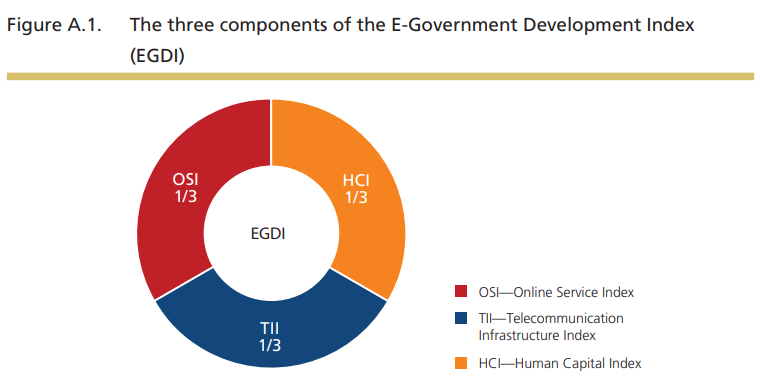
\includegraphics[width=1\linewidth]{figuras/egdi/egdi_componentes.png}
	\label{fig:egdi_componentes}
	\footnotesize{Fonte: \cite{ONU_EGDI_methodology}}
\end{figure}

A figura \ref{fig:boxplot_egov_global} contém um diagrama de caixa que representa o EGDI global.

\begin{figure}[H]
	\centering
	\caption{E-Government Development Index global em 2024}
	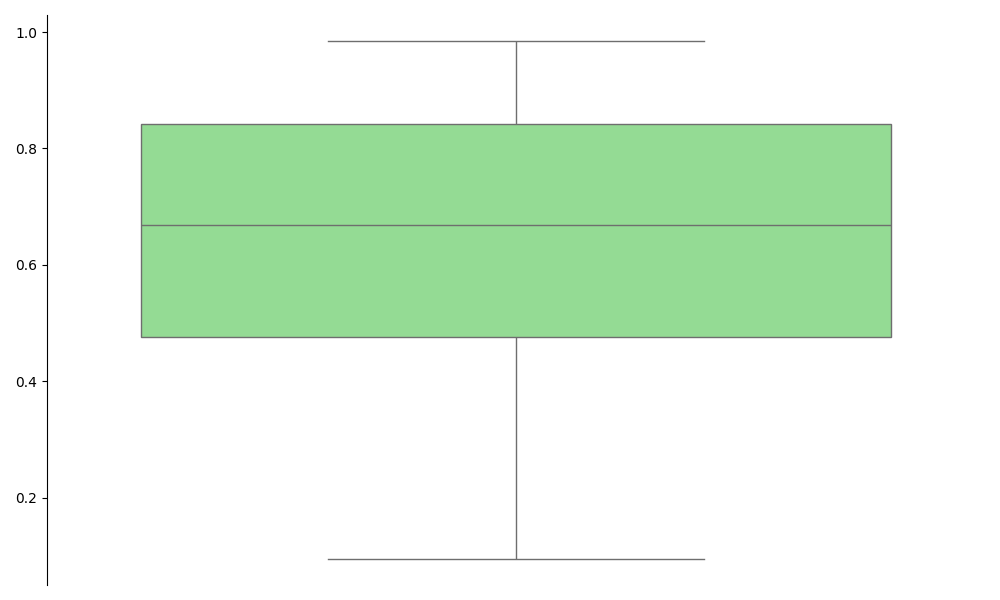
\includegraphics[width=1\linewidth]{figuras/egdi/boxplot_egov_global.png}
	\label{fig:boxplot_egov_global}
	\footnotesize{Fonte: baseado em \cite{ONU_EGDI_mapa}.}
\end{figure}

A linha central na caixa indica que a mediana do índice é de aproximadamente 0.65. A caixa em si, que representa os 50\% centrais dos dados, se estende de cerca de 0.48 a 0.83, mostrando a variação dos índices na maioria dos países. As linhas verticais, conhecidas como "bigodes", demonstram a amplitude total dos dados, que vai de aproximadamente 0.1 a quase 1.0. A distribuição do índice parece ser relativamente simétrica, sem um viés perceptível para valores mais altos ou mais baixos, e o gráfico não identifica a presença de valores discrepantes (outliers) extremos.

\section{E-Participation Index}
\label{epart}

\cite{ONU_EGDI} argumenta que o \textbf{E-Participation Index} deriva do EGDI como índice suplementar ao relatório \textbf{E-Government Survey}. Os componentes do índice são: \textbf{E-information}, \textbf{E-consultation} e \textbf{E-decision-making}. 

\textbf{E-information} fala sobre a facilitação da participação dos cidadãos via informações públicas e acesso a informação sem necessidade de pedido ou sob demanda. \textbf{E-consultation} diz respeito ao engajamento dos cidadãos em contribuições e deliberações sobre políticas publicas e serviços públicos. \textbf{E-decision-making} engloba o empoderamento dos cidadãos via a opção de coparticipação na elaboração de políticas e coprodução de componentes de serviços e entrega de modalidades.

\cite{ONU_EGDI} esclarece que o \textbf{E-Participation Index} de um país reflete os mecanismos do índice que são empregados pelo governo quando se faz comparações com todos outros países. 

O propósito dessa medição não é prescrever qualquer prática especificam, no entanto oferece perspectivas de como países diferentes estão usando ferramentas online para promover interação entre o governo e seu povo, bem como, entre as pessoas para benefícios de todos.

A figura \ref{fig:boxplot_epart_global} contém um diagrama de caixa que representa o \textbf{E-Participation Index} global.

\begin{figure}[H]
	\centering
	\caption{E-Participation Index global em 2024}
	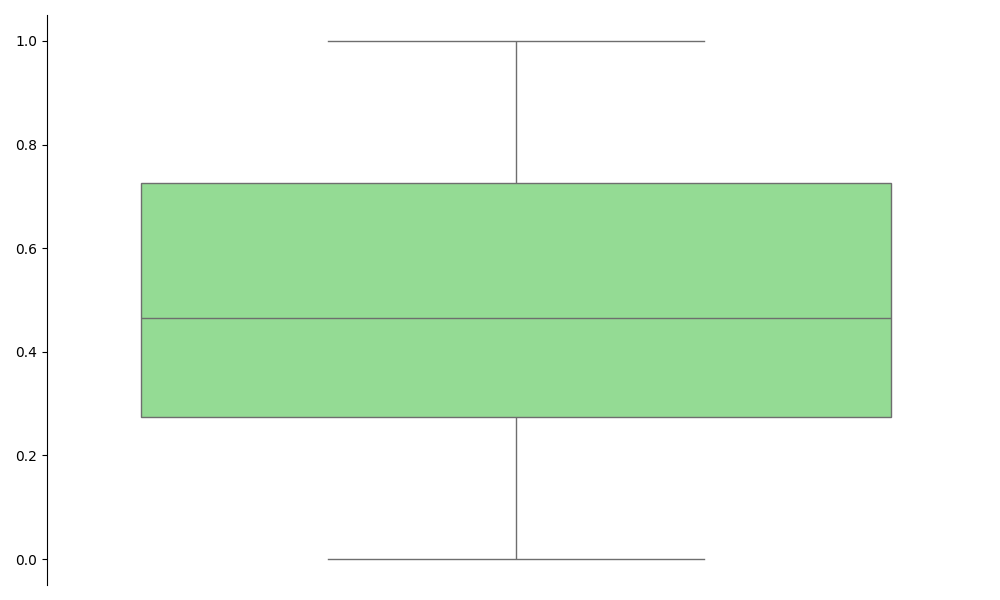
\includegraphics[width=1\linewidth]{figuras/egdi/boxplot_epart_global.png}
	\label{fig:boxplot_epart_global}
	\footnotesize{Fonte: baseado em \cite{ONU_EGDI_mapa}.}
\end{figure}

A figura \ref{fig:boxplot_epart_global} revela que a mediana do índice é de aproximadamente 0.47, indicando que metade dos países avaliados se encontra acima desse valor. A caixa do gráfico abrange o intervalo entre 0.28 e 0.72, onde estão concentrados 50\% dos países. A amplitude total dos índices é considerável, variando de 0.0 a 1.0. A distribuição se apresenta como relativamente simétrica, sem uma concentração significativa de países nas extremidades dos dados, e não há indícios de valores discrepantes (outliers).

\section{Online Service Index}
\label{osi}

A figura \ref{fig:boxplot_osi_global} contém um diagrama de caixa que representa o \textbf{E-Participation Index} global.

\begin{figure}[H]
	\centering
	\caption{Online Service Index global em 2024}
	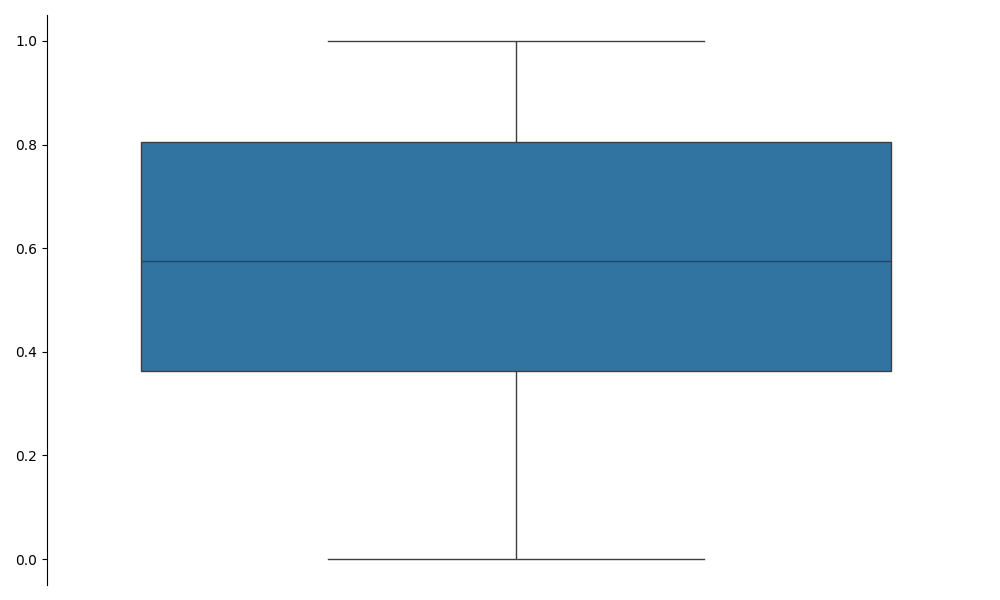
\includegraphics[width=1\linewidth]{figuras/egdi/boxplot_osi_global.png}
	\label{fig:boxplot_osi_global}
	\footnotesize{Fonte: baseado em \cite{ONU_EGDI_mapa}.}
\end{figure}

A figura \ref{fig:boxplot_osi_global} revela que a mediana do índice de serviços online é de aproximadamente 0.58. A caixa principal do gráfico indica que 50\% dos países têm índices que variam entre 0.38 e 0.81. A amplitude total dos dados é vasta, indo de 0.0 a 1.0, o que demonstra uma grande disparidade nos níveis de serviços online oferecidos globalmente. A distribuição dos dados é relativamente simétrica e, assim como nos gráficos anteriores, não há outliers visíveis.

\section{Human Capital Index em 2024}
\label{hci}

\cite{ONU_EGDI_methodology} afirma que \textbf{Human Capital Index} tem 4 indicadores: taxa bruta de matrícula, letramento adulto, anos de escolarização esperados e média de anos de escolaridade. 

A taxa bruta de matrícula é medida como a combinação entre a taxa de matrícula nas educações primárias, secundários e terciárias. Letramento adulto é medido como o percentual de pessoas com pelos menos 15 anos de idade que entendem e sabem ler e escrever um frase curta simples na sua vida padrão.

Os anos de escolarização esperados é o número total de anos de escolarização que crianças de certa idade podem esperar ter no futuro, presumindo que a probabilidade de a criança de qualquer idade estiver na escola correspondendo à idade da taxa de matrícula atual.

A média de anos de escolaridade fornece o número médio de anos de educação concluídos pela população adulta de um país (25 anos ou mais), excluindo os anos gastos repetindo séries. 

A figura \ref{fig:boxplot_hci_global} contém um diagrama de caixa que representa o \textbf{E-Participation Index} global.

\begin{figure}[H]
	\centering
	\caption{Human Capital Index global em 2024}
	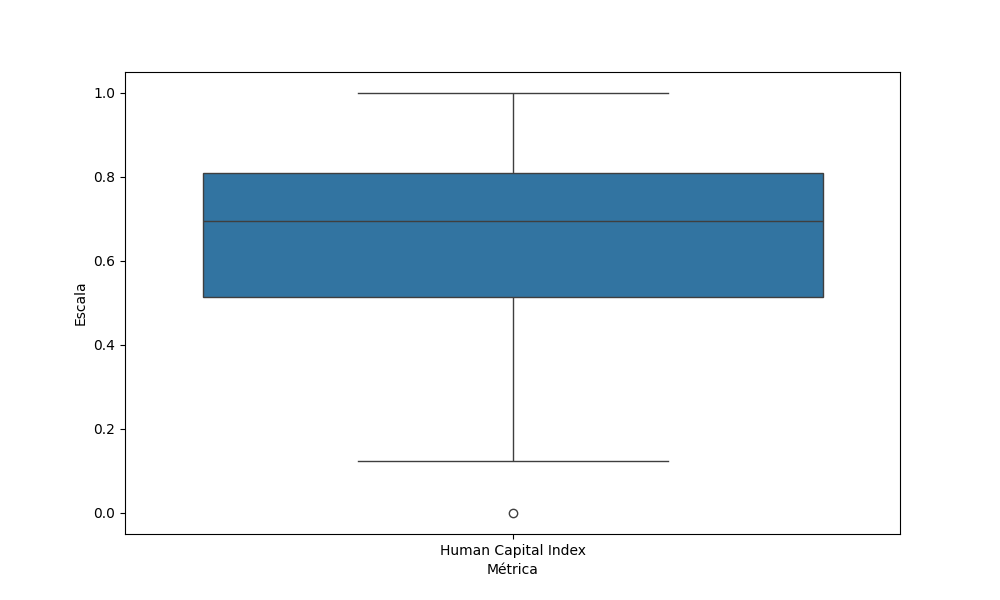
\includegraphics[width=1\linewidth]{figuras/egdi/boxplot_hci_global.png}
	\label{fig:boxplot_hci_global}
	\footnotesize{Fonte: baseado em \cite{ONU_EGDI_mapa}.}
\end{figure}

A figura \ref{fig:boxplot_hci_global} mostra que a mediana do índice de capital humano é de aproximadamente 0.70. A caixa principal, que concentra os 50\% centrais dos dados, indica que a maioria dos países tem um índice que varia entre 0.52 e 0.81. A amplitude dos dados é ampla, indo de cerca de 0.13 a 1.0. A distribuição se apresenta como relativamente simétrica, e, diferentemente dos gráficos anteriores, este diagrama aponta a existência de um outlier, um valor discrepante isolado, localizado próximo ao zero no eixo vertical, indicando um país com um índice de capital humano excepcionalmente baixo em comparação com os demais.

\section{Telecommunication Infrastructure Index em 2024}
\label{tii}

\cite{ONU_EGDI_methodology} afirma que o \textbf{Telecommunication Infrastructure Index} tem 5 componentes: usuário de internet, assinatura de banda larga fixa, assinatura de banda larga sem fio, assinatura de telefone fixo e assinatura de dados móveis.

A figura \ref{fig:boxplot_tci_global} contém um diagrama de caixa que representa o \textbf{E-Participation Index} global.

\begin{figure}[H]
	\centering
	\caption{Telecommunication Infrastructure Index global em 2024}
	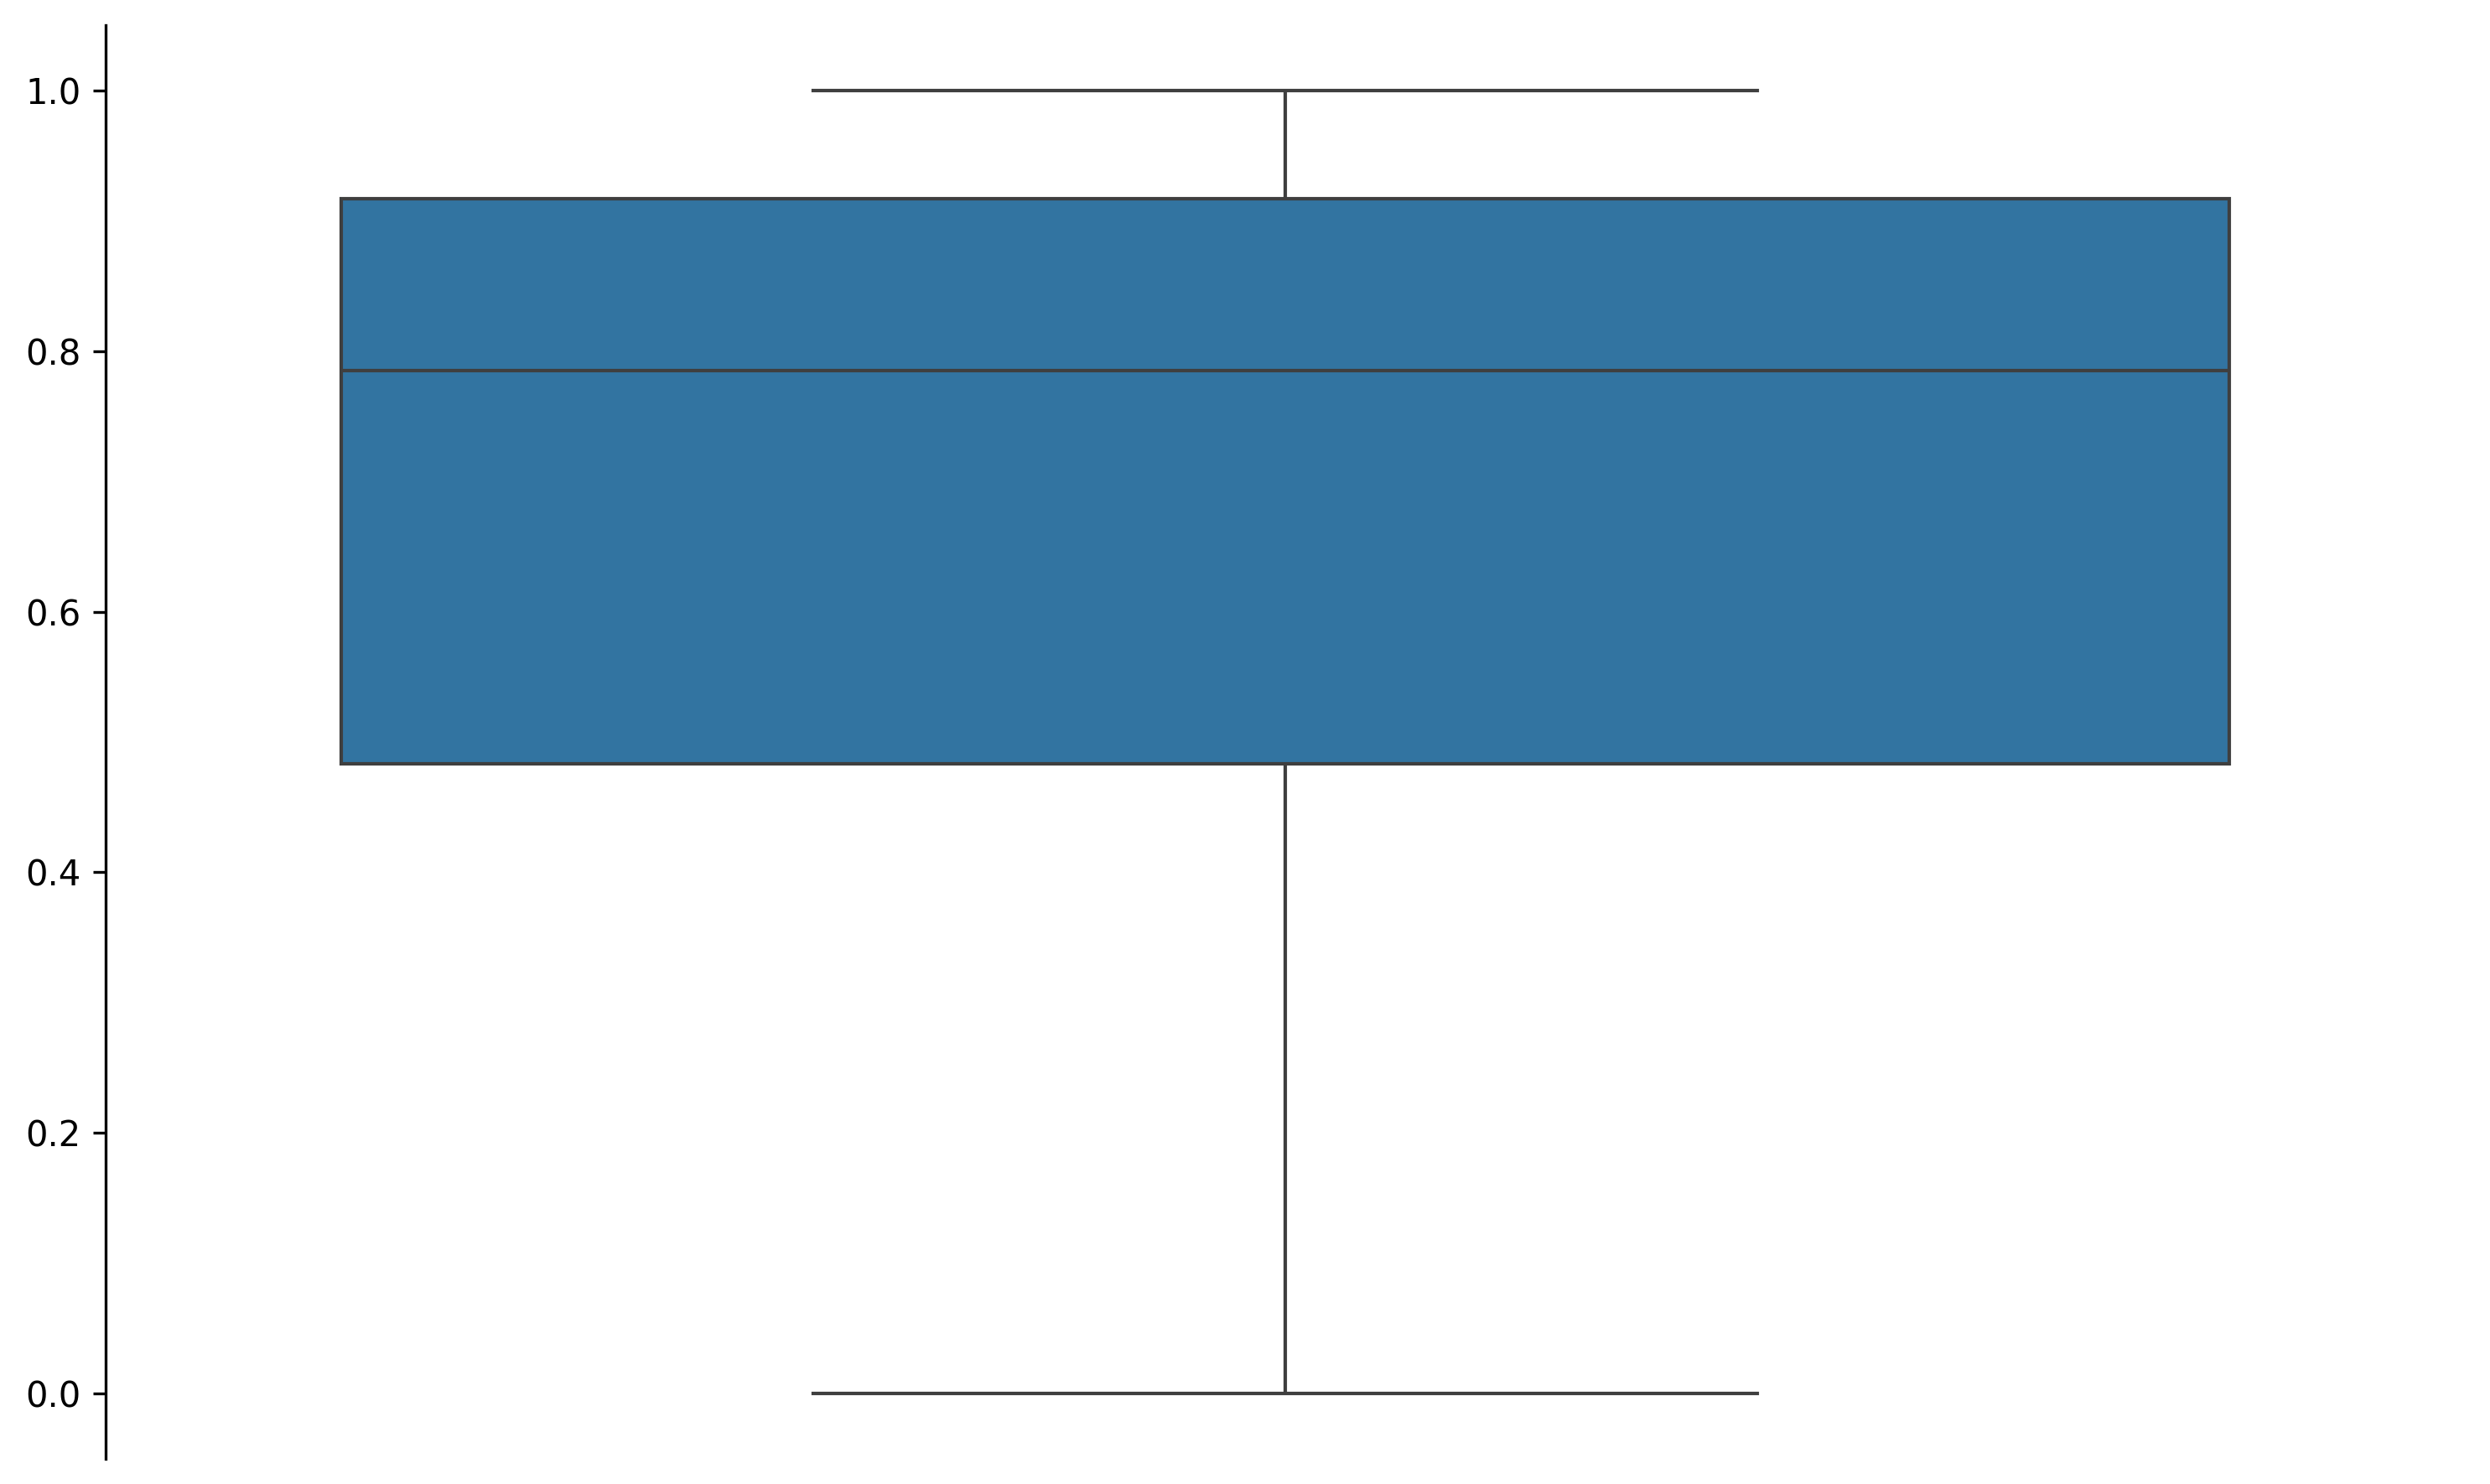
\includegraphics[width=1\linewidth]{figuras/egdi/boxplot_tci_global.png}
	\label{fig:boxplot_tci_global}
	\footnotesize{Fonte: baseado em \cite{ONU_EGDI_mapa}.}
\end{figure}

A figura \ref{fig:boxplot_tci_global} mostra que a mediana do índice de infraestrutura de telecomunicações está em cerca de 0.80, indicando que metade dos países possui um índice superior a esse valor. A caixa do gráfico, que representa os 50\% centrais dos dados, abrange o intervalo entre aproximadamente 0.50 e 0.90. A amplitude total dos dados varia de 0.0 a 1.0. A distribuição dos dados é relativamente simétrica e, assim como na maioria dos gráficos anteriores, não há outliers visíveis.

\section{Coeficiente de correlação: EGDI e E-Participation comparadas com outras variáveis}

Ao analisar os dados do \href{https://publicadministration.un.org/egovkb/en-us/About/Overview/-E-Government-Development-Index}{EGDI}, foi notado que tanto democracias consolidadas, quanto autocracias tem um EGDI alto. O critério para entender quais países são democráticos ou autocráticos foi a figura \ref{fig:electoral-democracy-index}. 

\begin{figure}[H]
	\centering
	\caption{Índice da democracia eleitoral}
	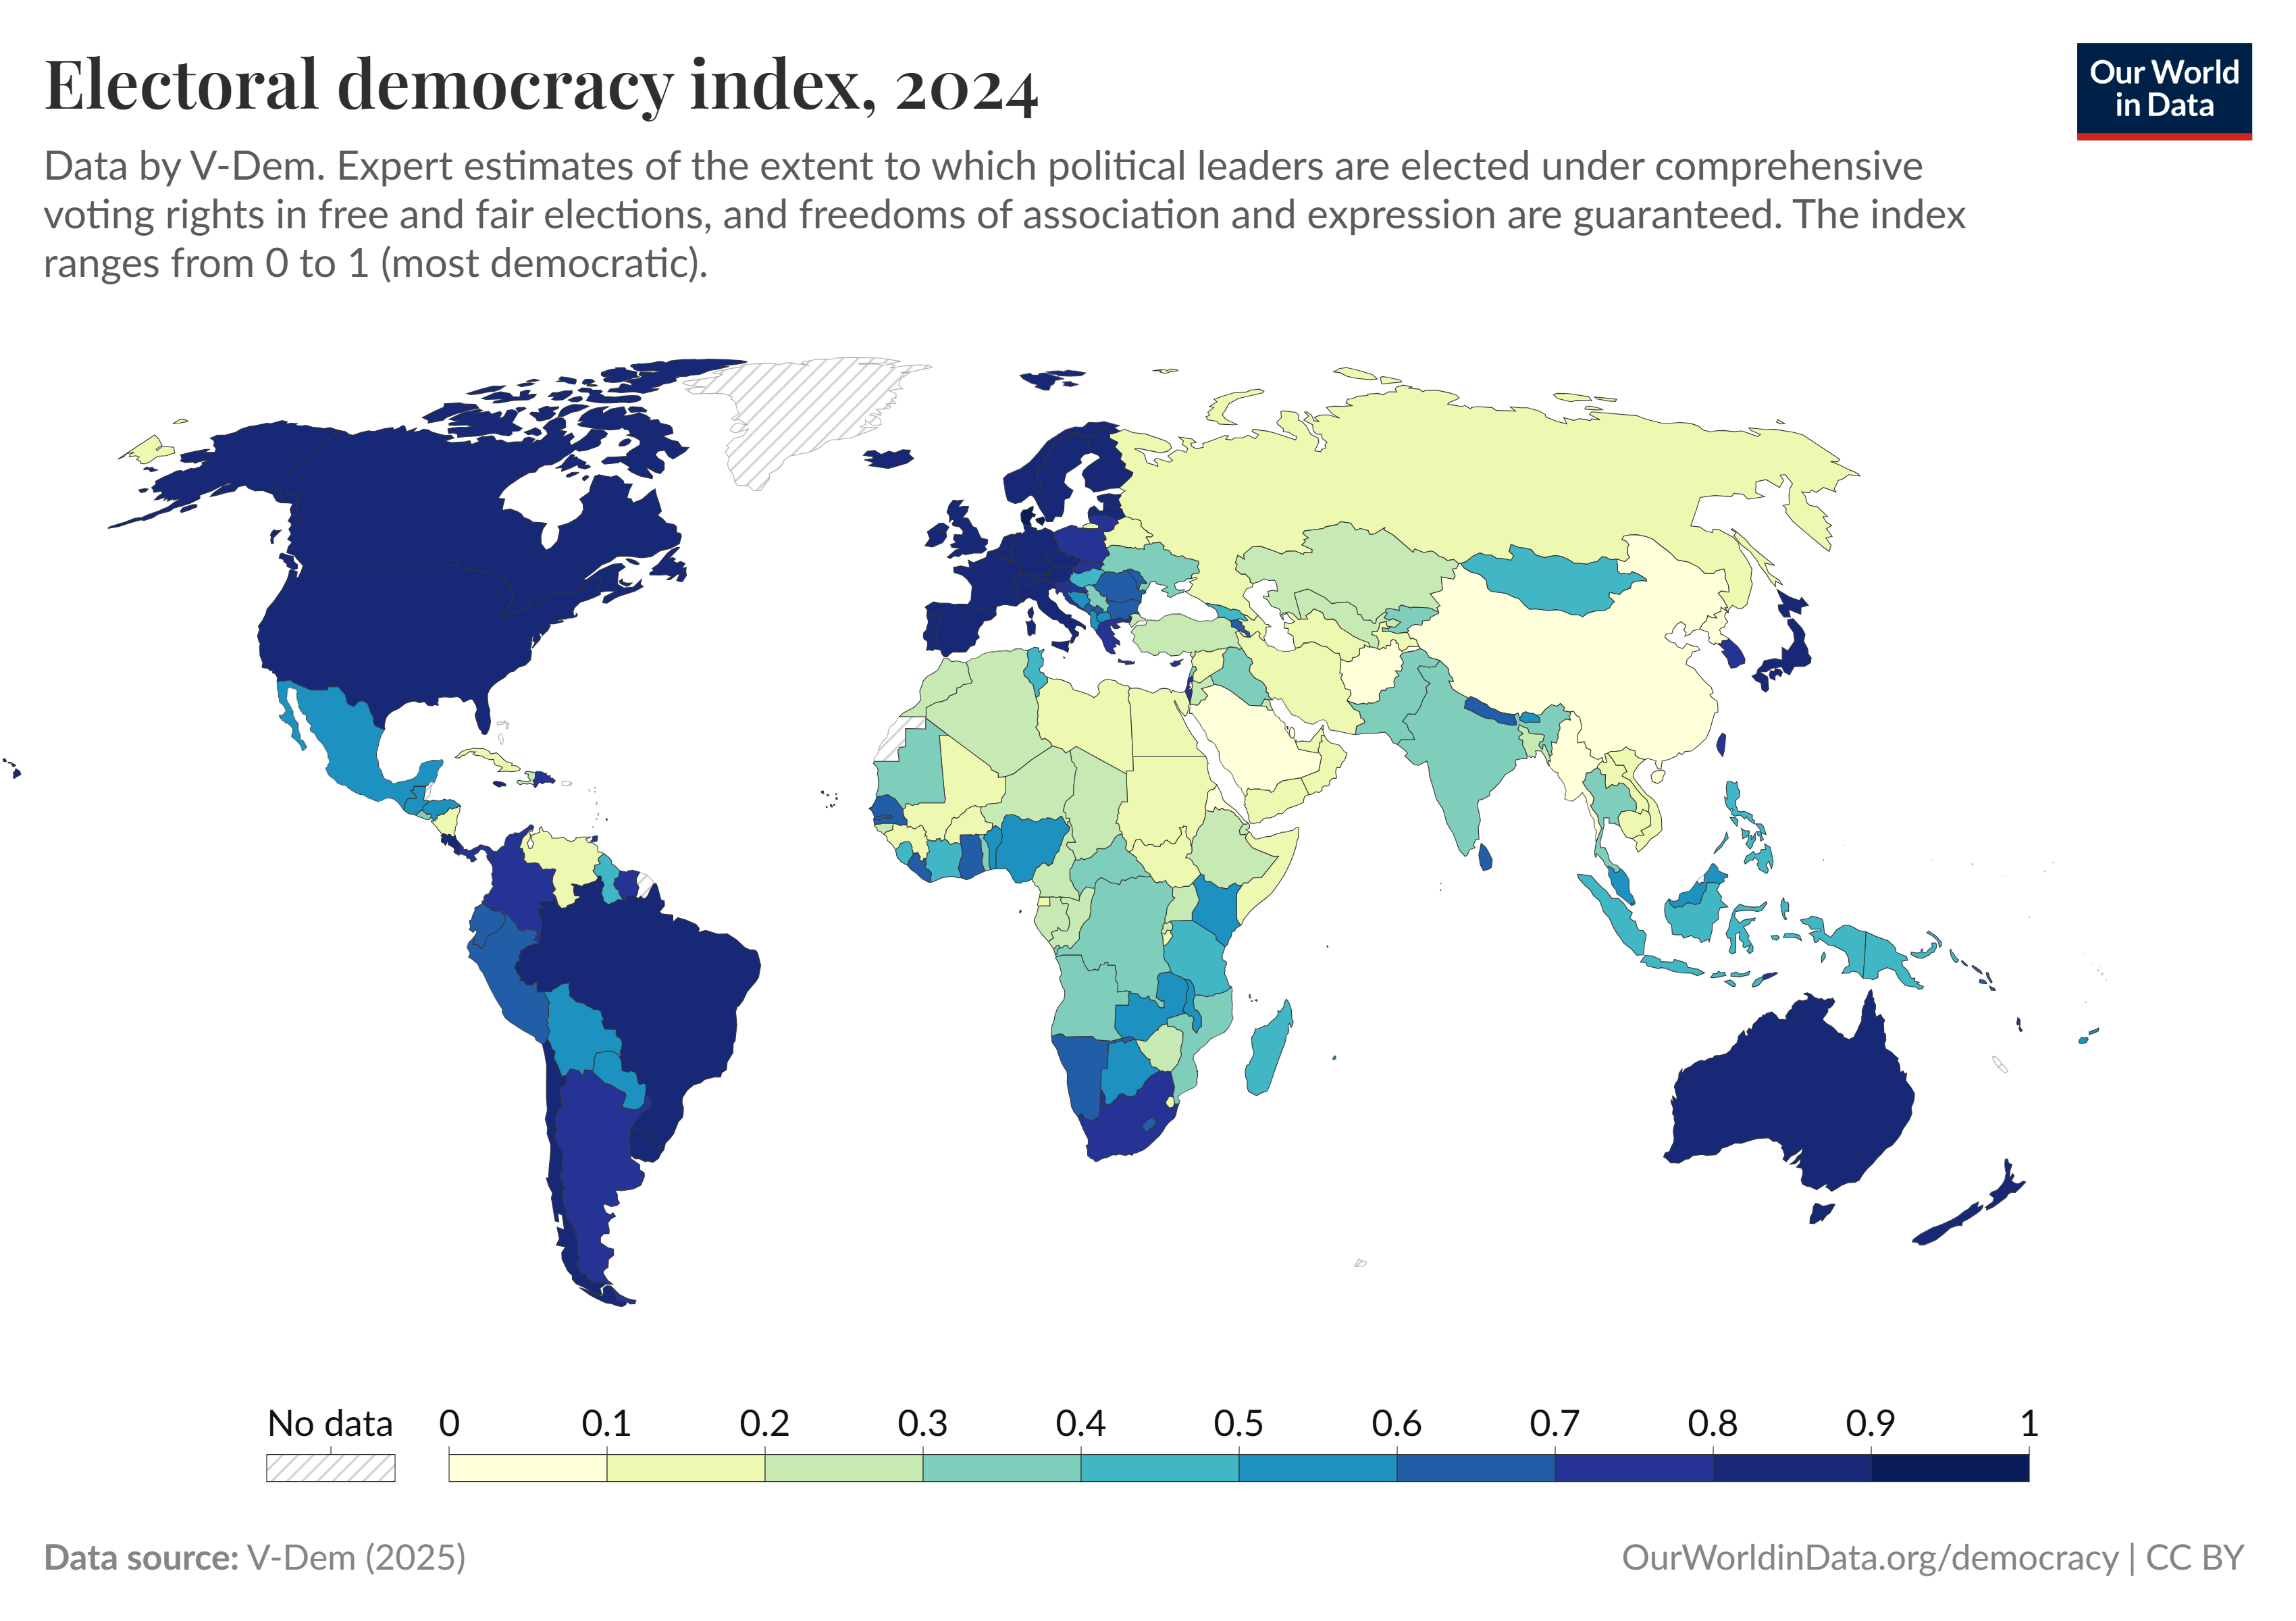
\includegraphics[width=1\linewidth]{figuras/democracia/electoral-democracy-index.png}
	\label{fig:electoral-democracy-index}
	\footnotesize{Fonte: \cite{electoral_democracy_index}}
\end{figure}

Nota-se que o Brasil é considerado uma democracia eleitoral, estando na minoria numérica de países democráticas (88), conforme exposto por \cite{nord2025democracy}, contra 91 autocracias no ano de 2025, haja vista o relatótio \href{https://www.v-dem.net/documents/60/V-dem-dr__2025_lowres.pdf}{DEMOCRACY REPORT 2025: 25 Years of Autocratization – Democracy Trumped?}

Outro fator chamou atenção: há EGDI alto em países tanto autocráticos, quanto democráticos que têm PIB \textit{per capita} alto, conforme comparação inicial dos \href{https://data.worldbank.org/indicator/NY.GDP.PCAP.PP.KD}{com o PIB \textit{per capita} dos países}. 

Adicionalmente, ao avaliar o gasto públicos dos governos apresentado pela OECD e resumido na figura \ref{fig:government-spending-by-function}, um detalhe foi chamativo.

\begin{figure}[H]
	\centering
	\caption{Gastos gerais governamentais (\% do PIB)}
	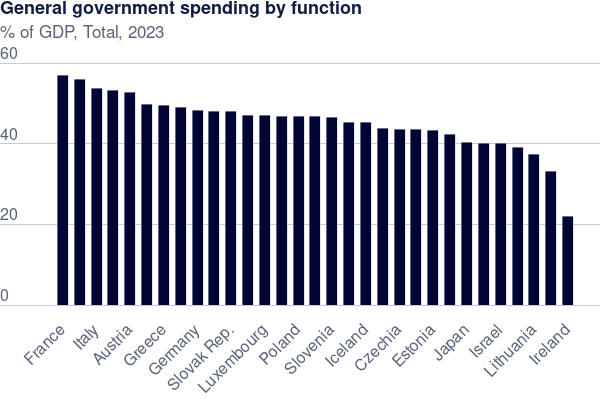
\includegraphics[width=1\linewidth]{figuras/government_spending/government-spending-by-function}
	\label{fig:government-spending-by-function}
	\footnotesize{Fonte: \cite{global_gov_spending_function}}
\end{figure}

Notou-se que os páises democráticos (membros da OECD) que têm EGDI altos tem, coincidentemente, altos gastos públicos e que eles representam parte considerável do PIB. A França e a Itália lideram com uma pequena diferença da 2ª para a 1ª. Outro fato é notório é maioria dos países gastam mais de 40\% do PIB.

Com base nos parágrafos anteriores, um questionamento surgiu: qual é relação entre EGDI e \textbf{E-Participation Index} com o índice de democracia eleitoral do \href{https://www.v-dem.net/}{V-Dem}, com o PIB \textit{per capita} e com o gasto governamental como porcentagem do PIB. Para descobrir qual tipo de coeficiente de correlação usar, fez-se diagramas de dispersão. Caso haja linearidade, usar-se-á Pearson; caso contrário Spearman.

\subsection{Análise geral com EGDI e E-Participation Index}

Analisar-se-á o aspecto geral usando o EGDI e o E-Participation Index, estudando como essas variáveis se comportam em diagramas de dispersão e coeficientes de correlação quando comparada com outras variáveis.

\subsubsection{EGDI e PIB \textit{per capita} PPC}

\begin{figure}[H]
	\centering
	\caption{Diagrama de Dispensao: EGDI e PIB \textit{per capita} PPC}
	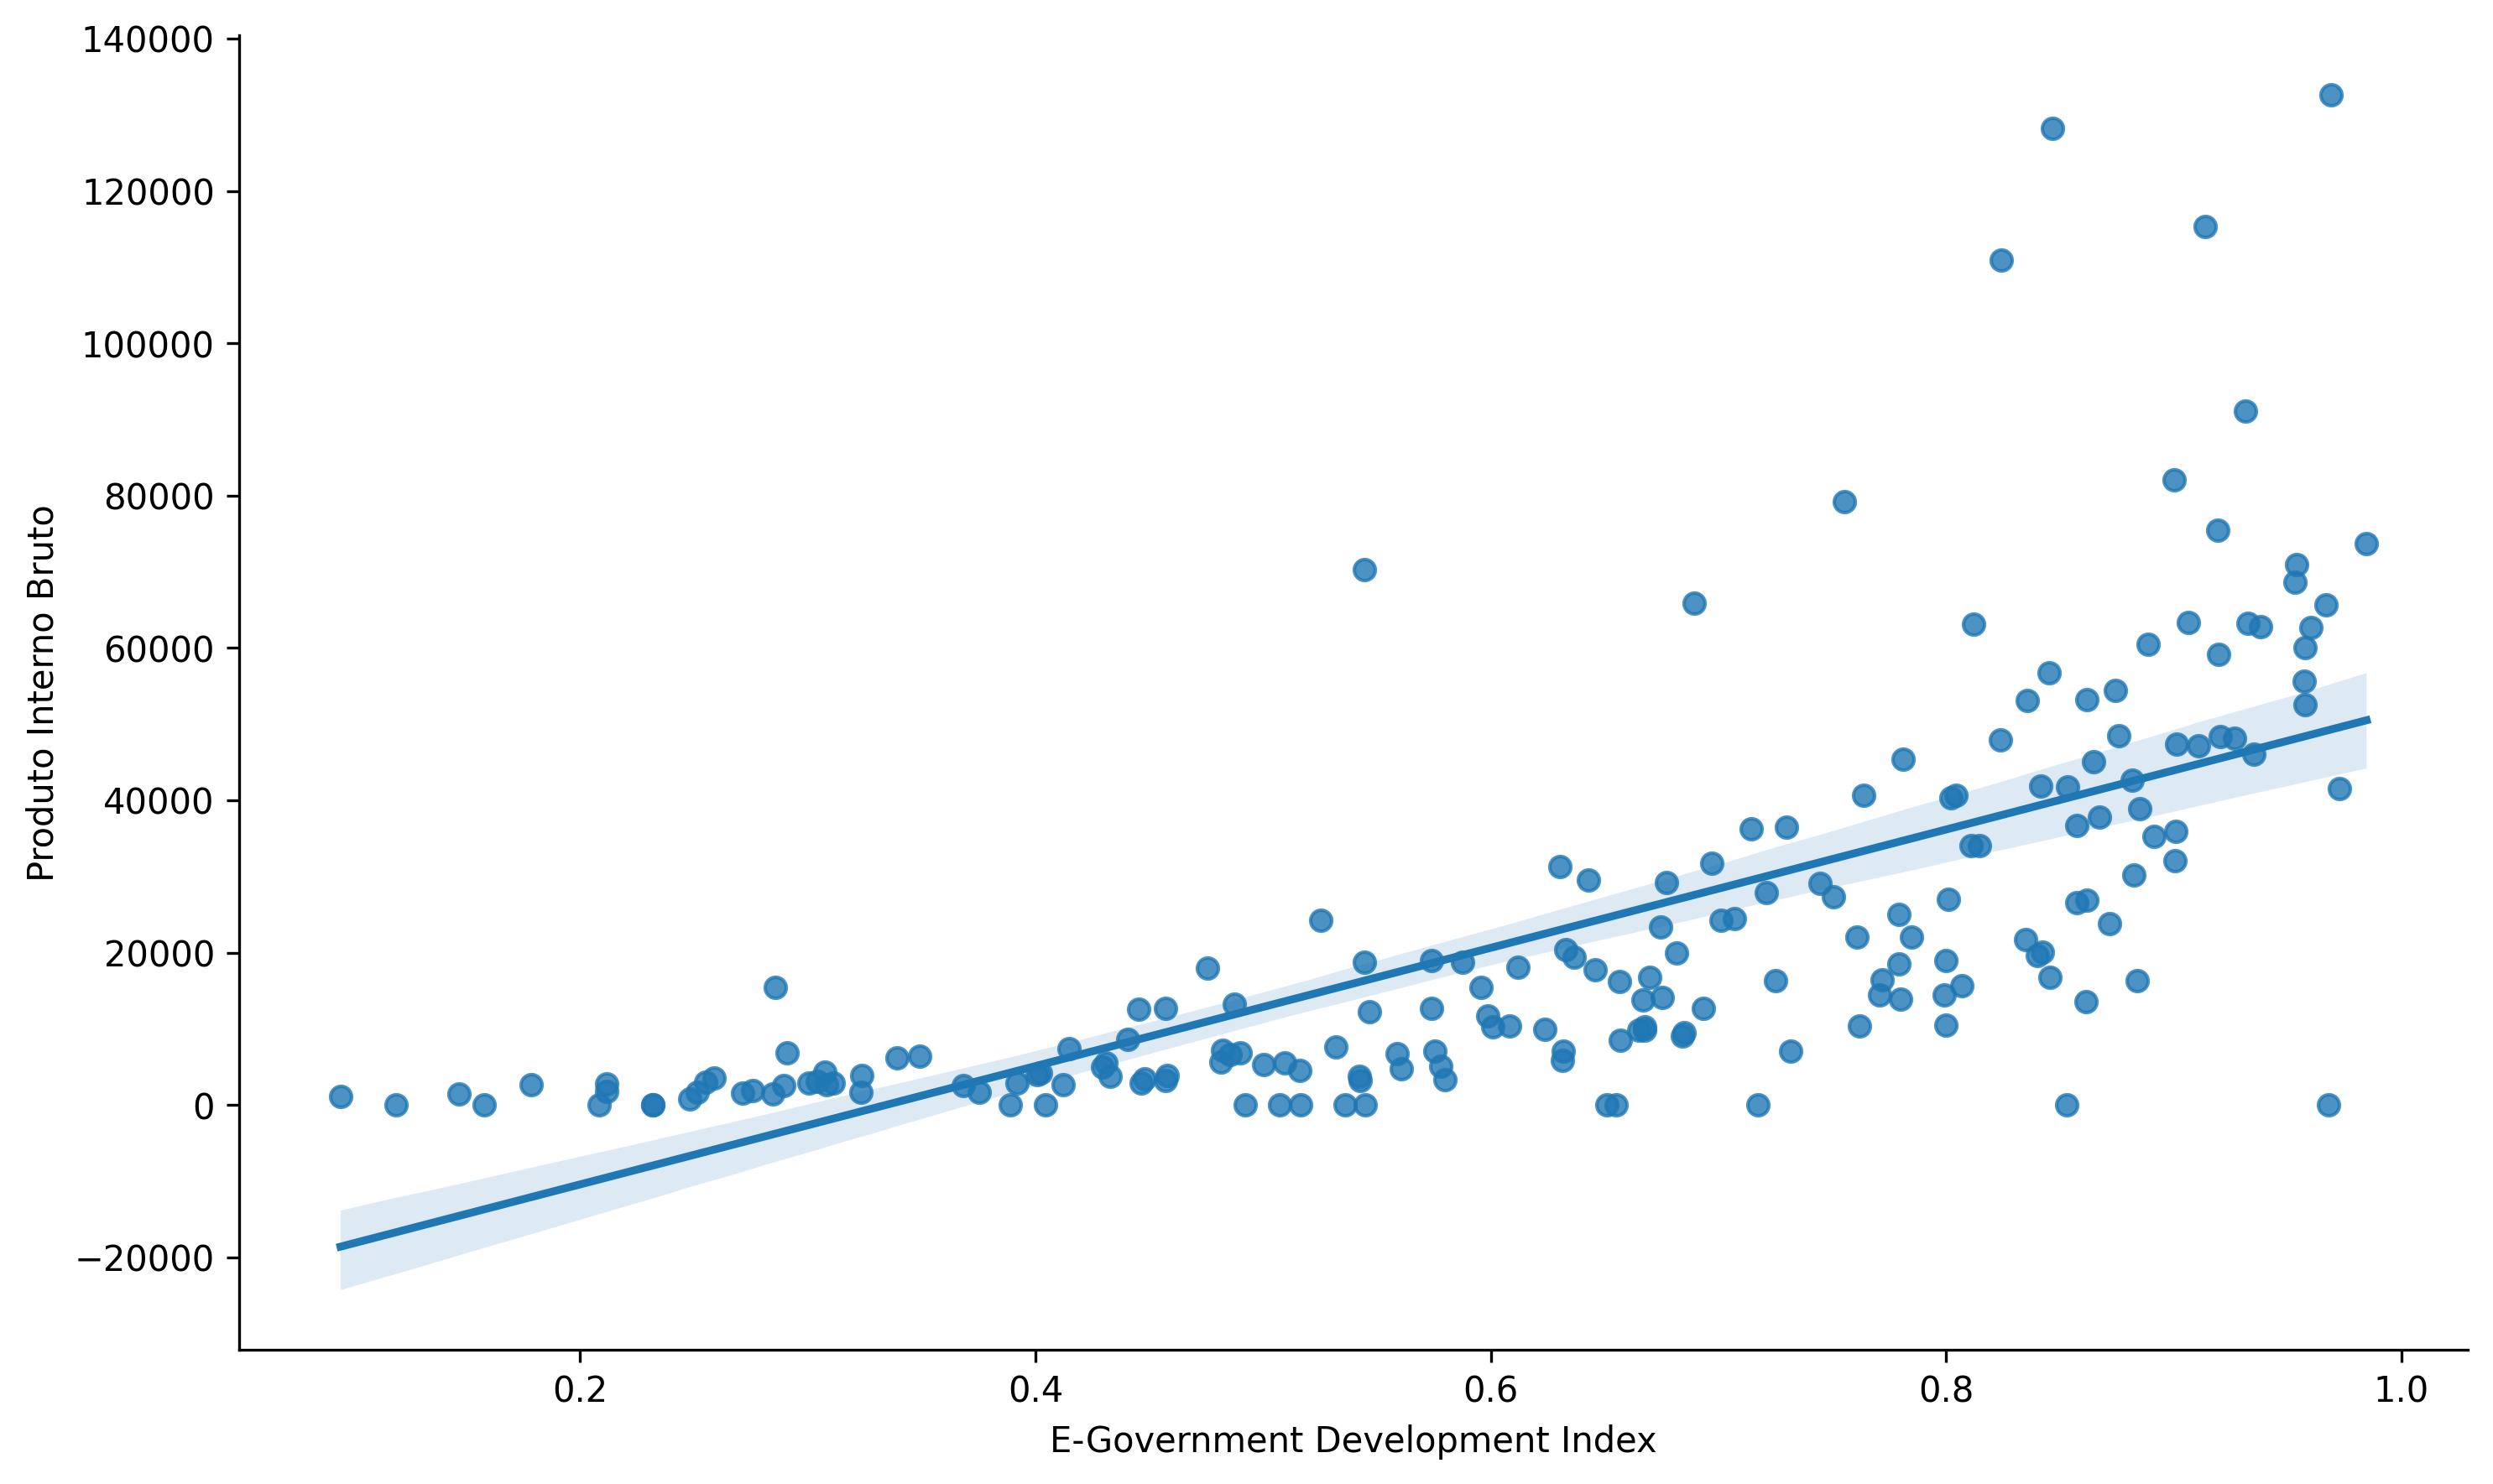
\includegraphics[width=1\linewidth]{figuras/egdi/dispensao_egov_pib}
	\label{fig:dispensao_egov_pib}
	\footnotesize{Fonte: \cite{ONU_EGDI} e \cite{WB_pib_per_capita_países}}
\end{figure}

Para compreender melhor o diagrama de dispersão, foi usado o coeficiente de correlação de Spearman. A sua escolha foi motivada pela grande presença de pontos extremos. O coeficiente de correlação encontrada foi 0.82. Devido ao coeficiente, os PIB \textit{per capita} PPC e o \textbf{E-Government Index} tendem a crescer juntos.

\subsubsection{E-Participation Index e PIB \textit{per capita} PPC}

\begin{figure}[H]
	\centering
	\caption{Diagrama de Dispensao: E-Participation Index e PIB \textit{per capita} PPC}
	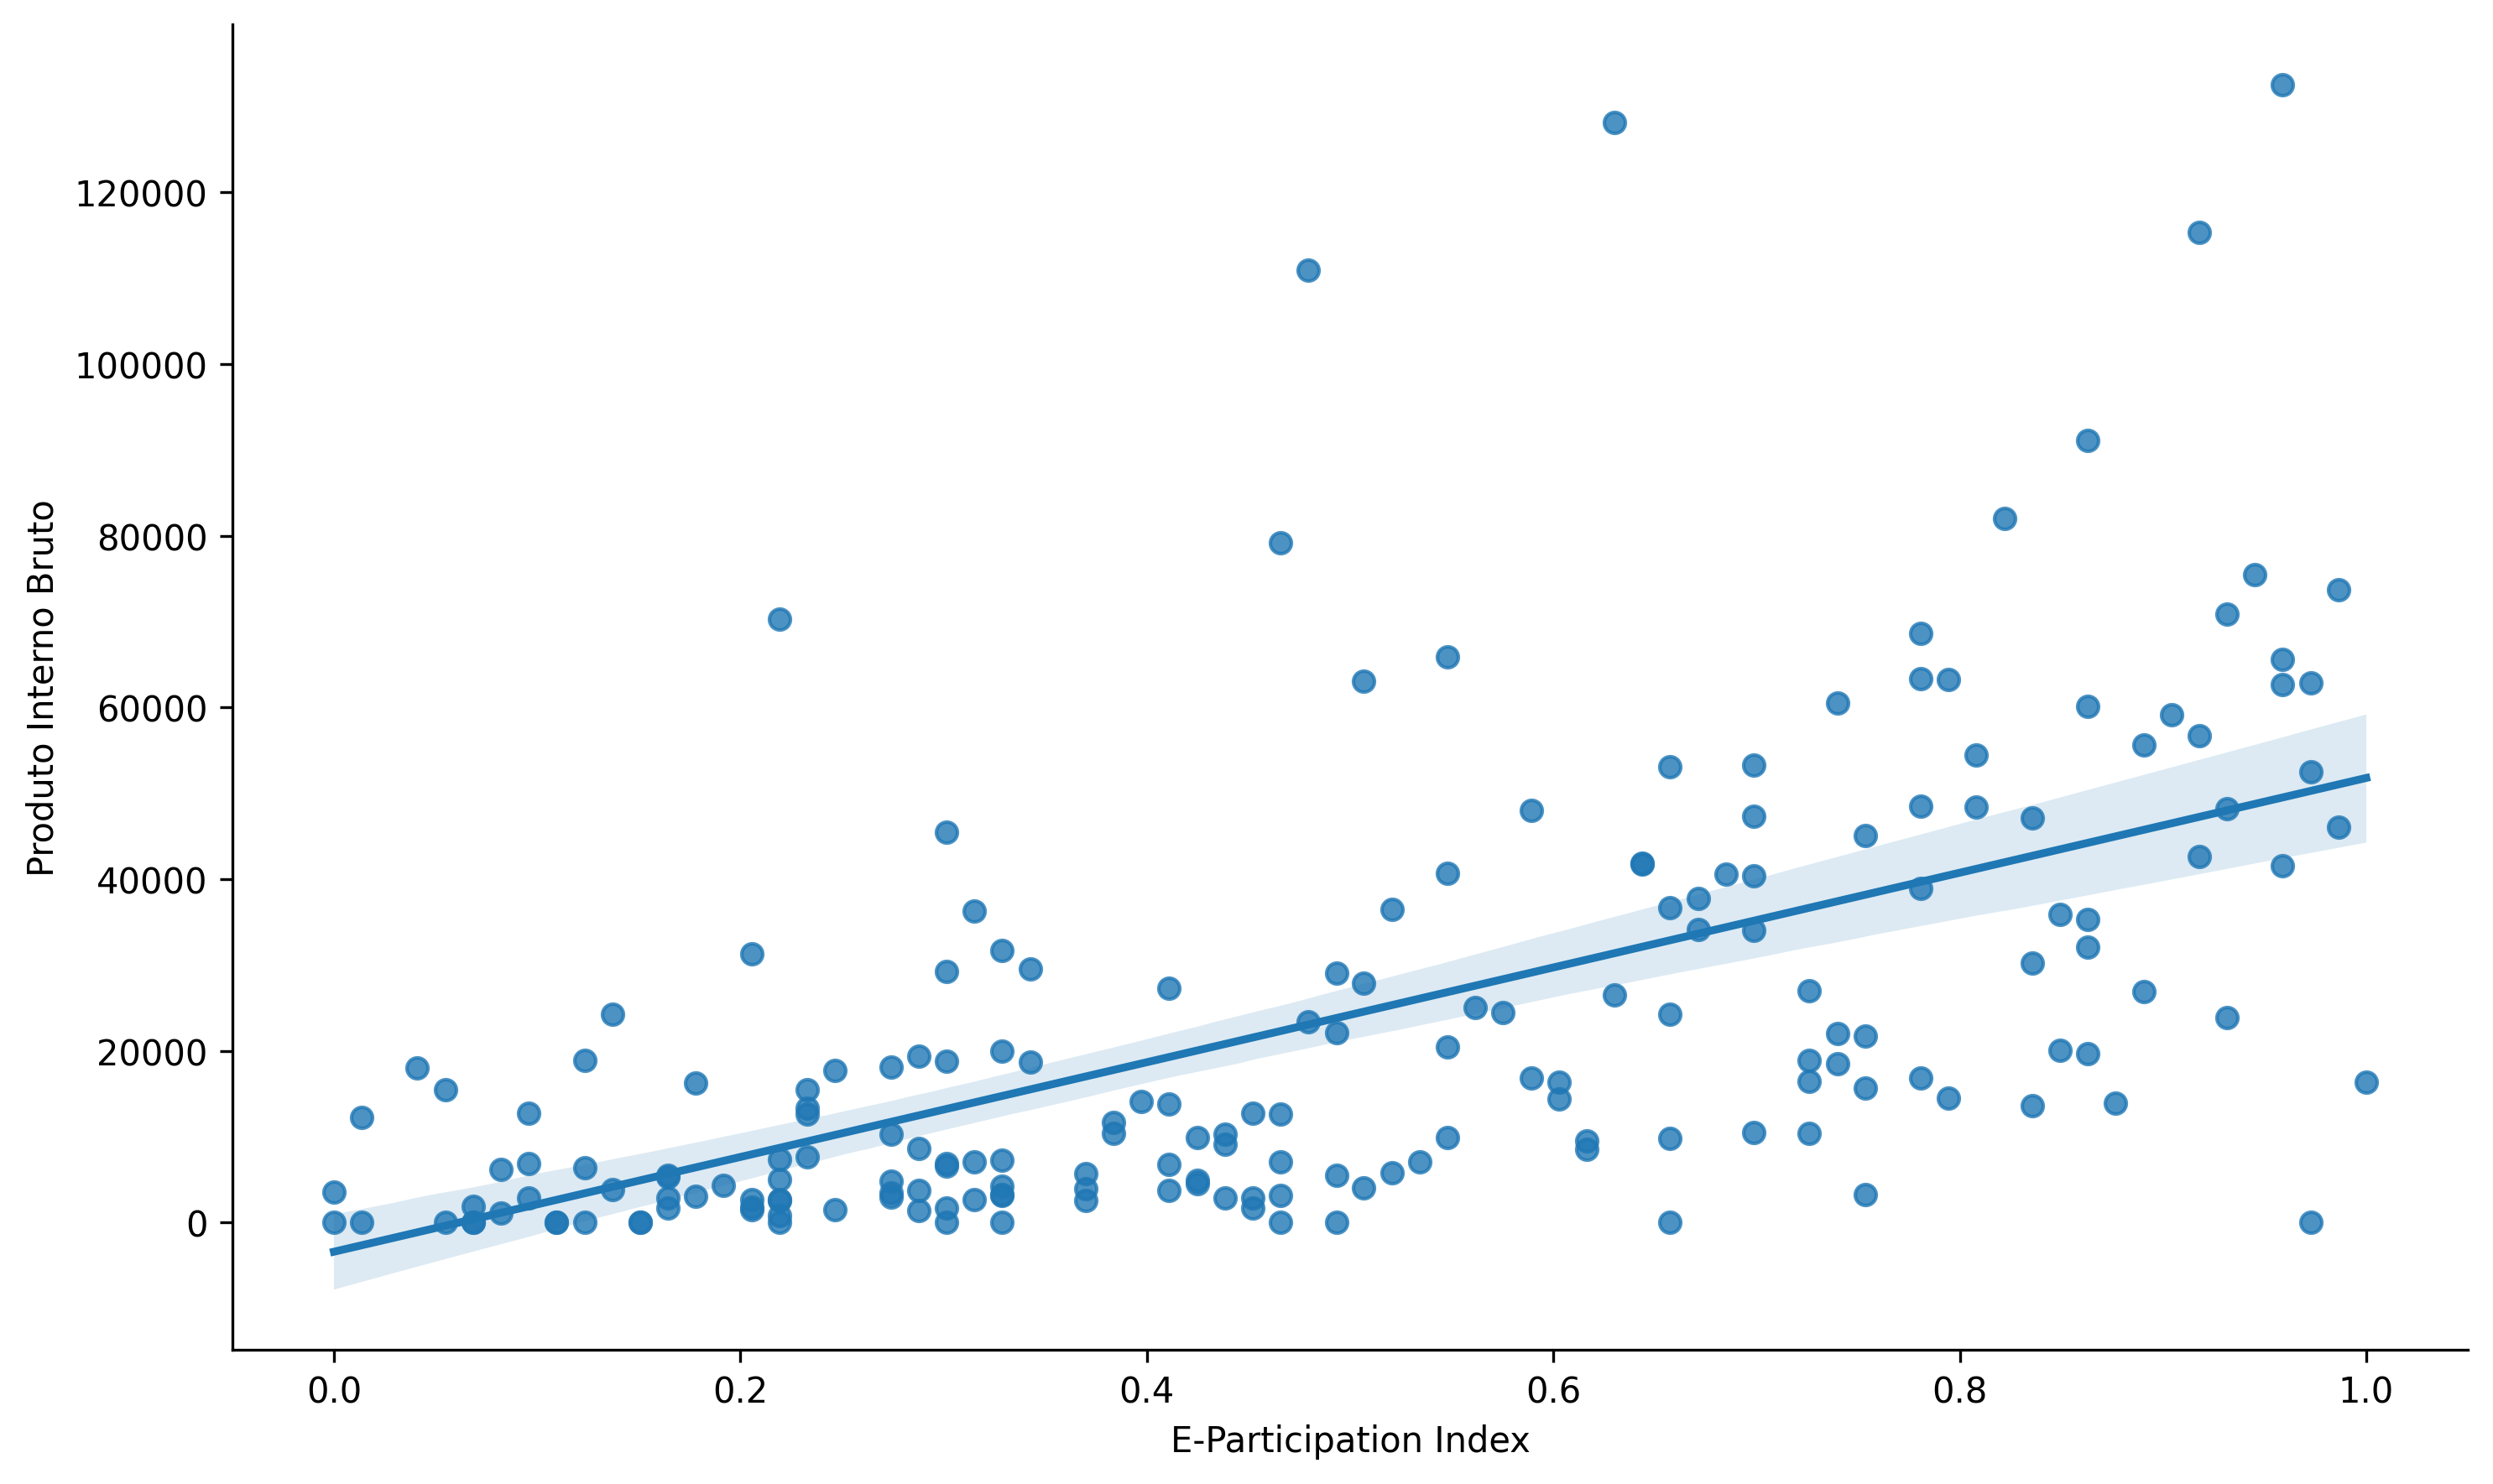
\includegraphics[width=1\linewidth]{figuras/egdi/dispensao_epart_pib}
	\label{fig:dispensao_epart_pib}
	\footnotesize{Fonte: \cite{ONU_EGDI_mapa} e \cite{WB_pib_per_capita_países}}
\end{figure}

Para compreender melhor o diagrama de dispersão, foi usado o coeficiente de correlação de Spearman. A sua escolha foi motivada pela grande presença de pontos extremos. O coeficiente de correlação encontrada foi 0.67. Devido ao coeficiente, os PIB \textit{per capita} PPC e o \textbf{E-Participation Index} tendem a crescer juntos.

\subsubsection{EGDI e índice de democracia eleitoral}

\begin{figure}[H]
	\centering
	\caption{Diagrama de Dispensao: EGDI e índice de democracia eleitoral}
	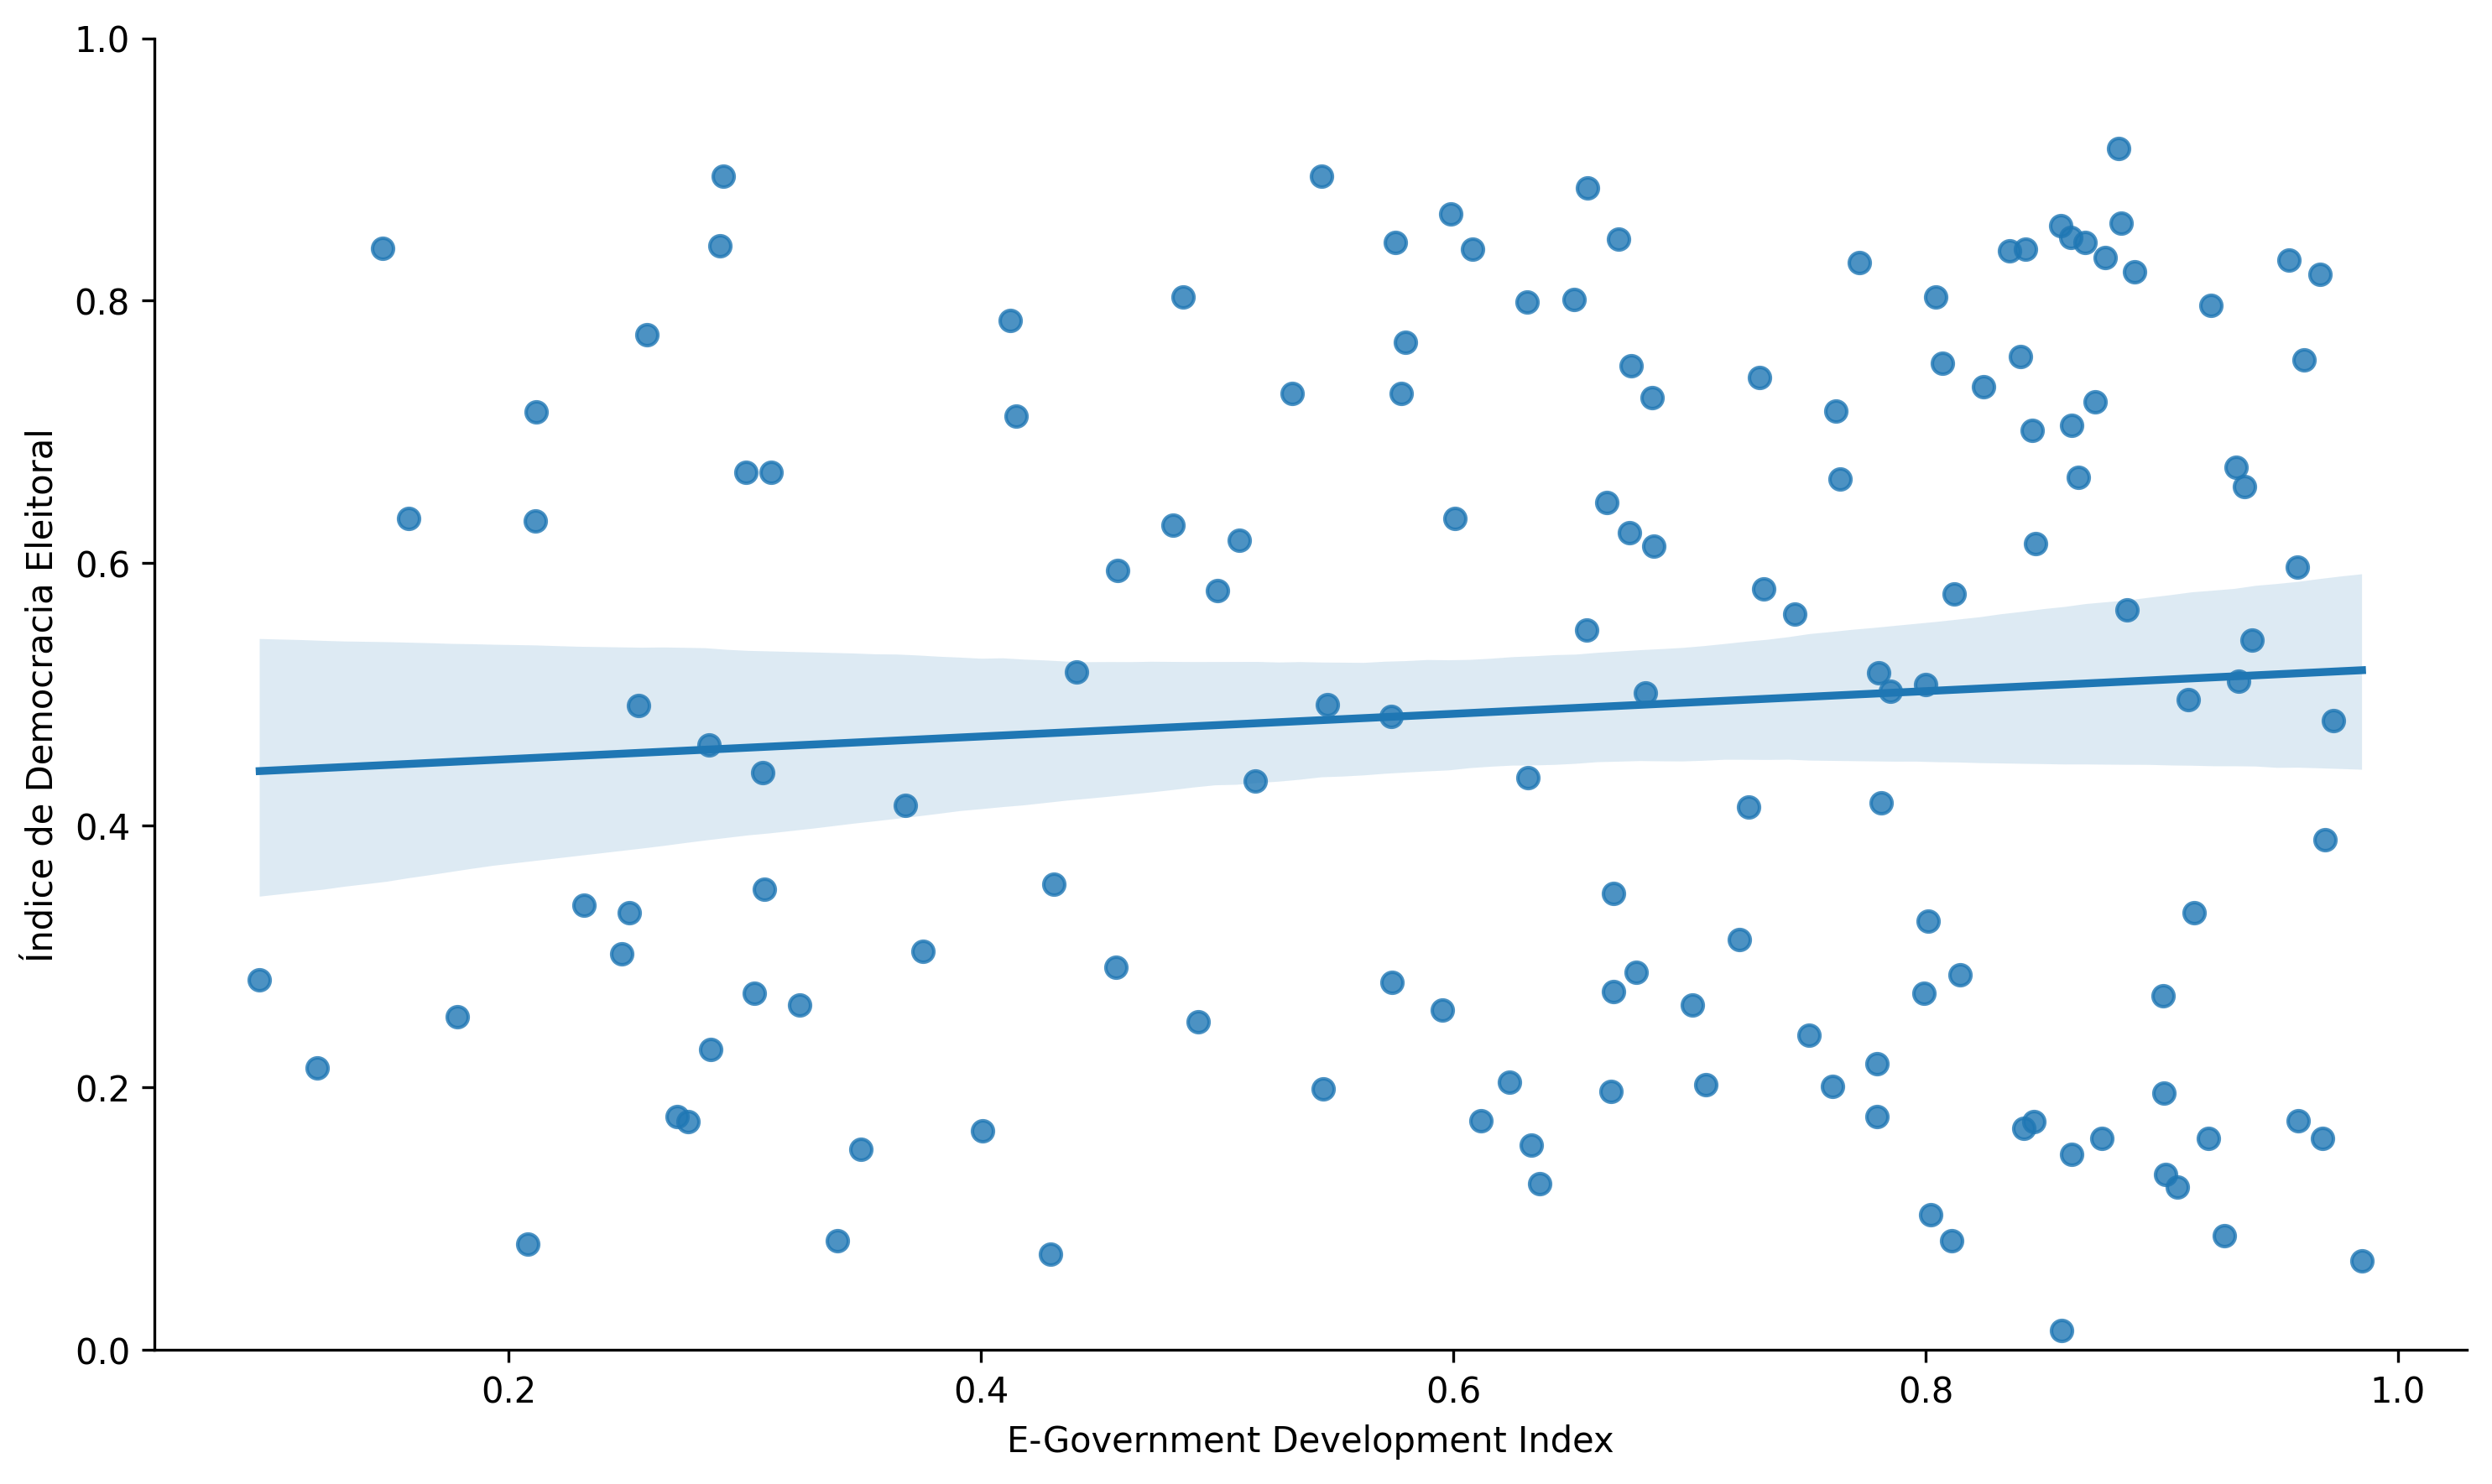
\includegraphics[width=1\linewidth]{figuras/egdi/dispersao_egov_indicedemocracia}
	\label{fig:dispersao_egov_indicedemocracia}
	\footnotesize{Fonte: \cite{ONU_EGDI} e \cite{electoral_democracy_index}}
\end{figure}

Para compreender melhor o diagrama de dispersão, foi usado o coeficiente de correlação de Spearman. A sua escolha foi motivada pela grande presença de pontos extremos. O coeficiente de correlação encontrada foi 0.04. Os índice de democracia eleitoral e o \textbf{E-Government Index} são variáveis independentes.

\subsubsection{E-Participation Index e índice de democracia eleitoral}

\begin{figure}[H]
	\centering
	\caption{Diagrama de Dispensao: E-Participation Index e índice de democracia eleitoral}
	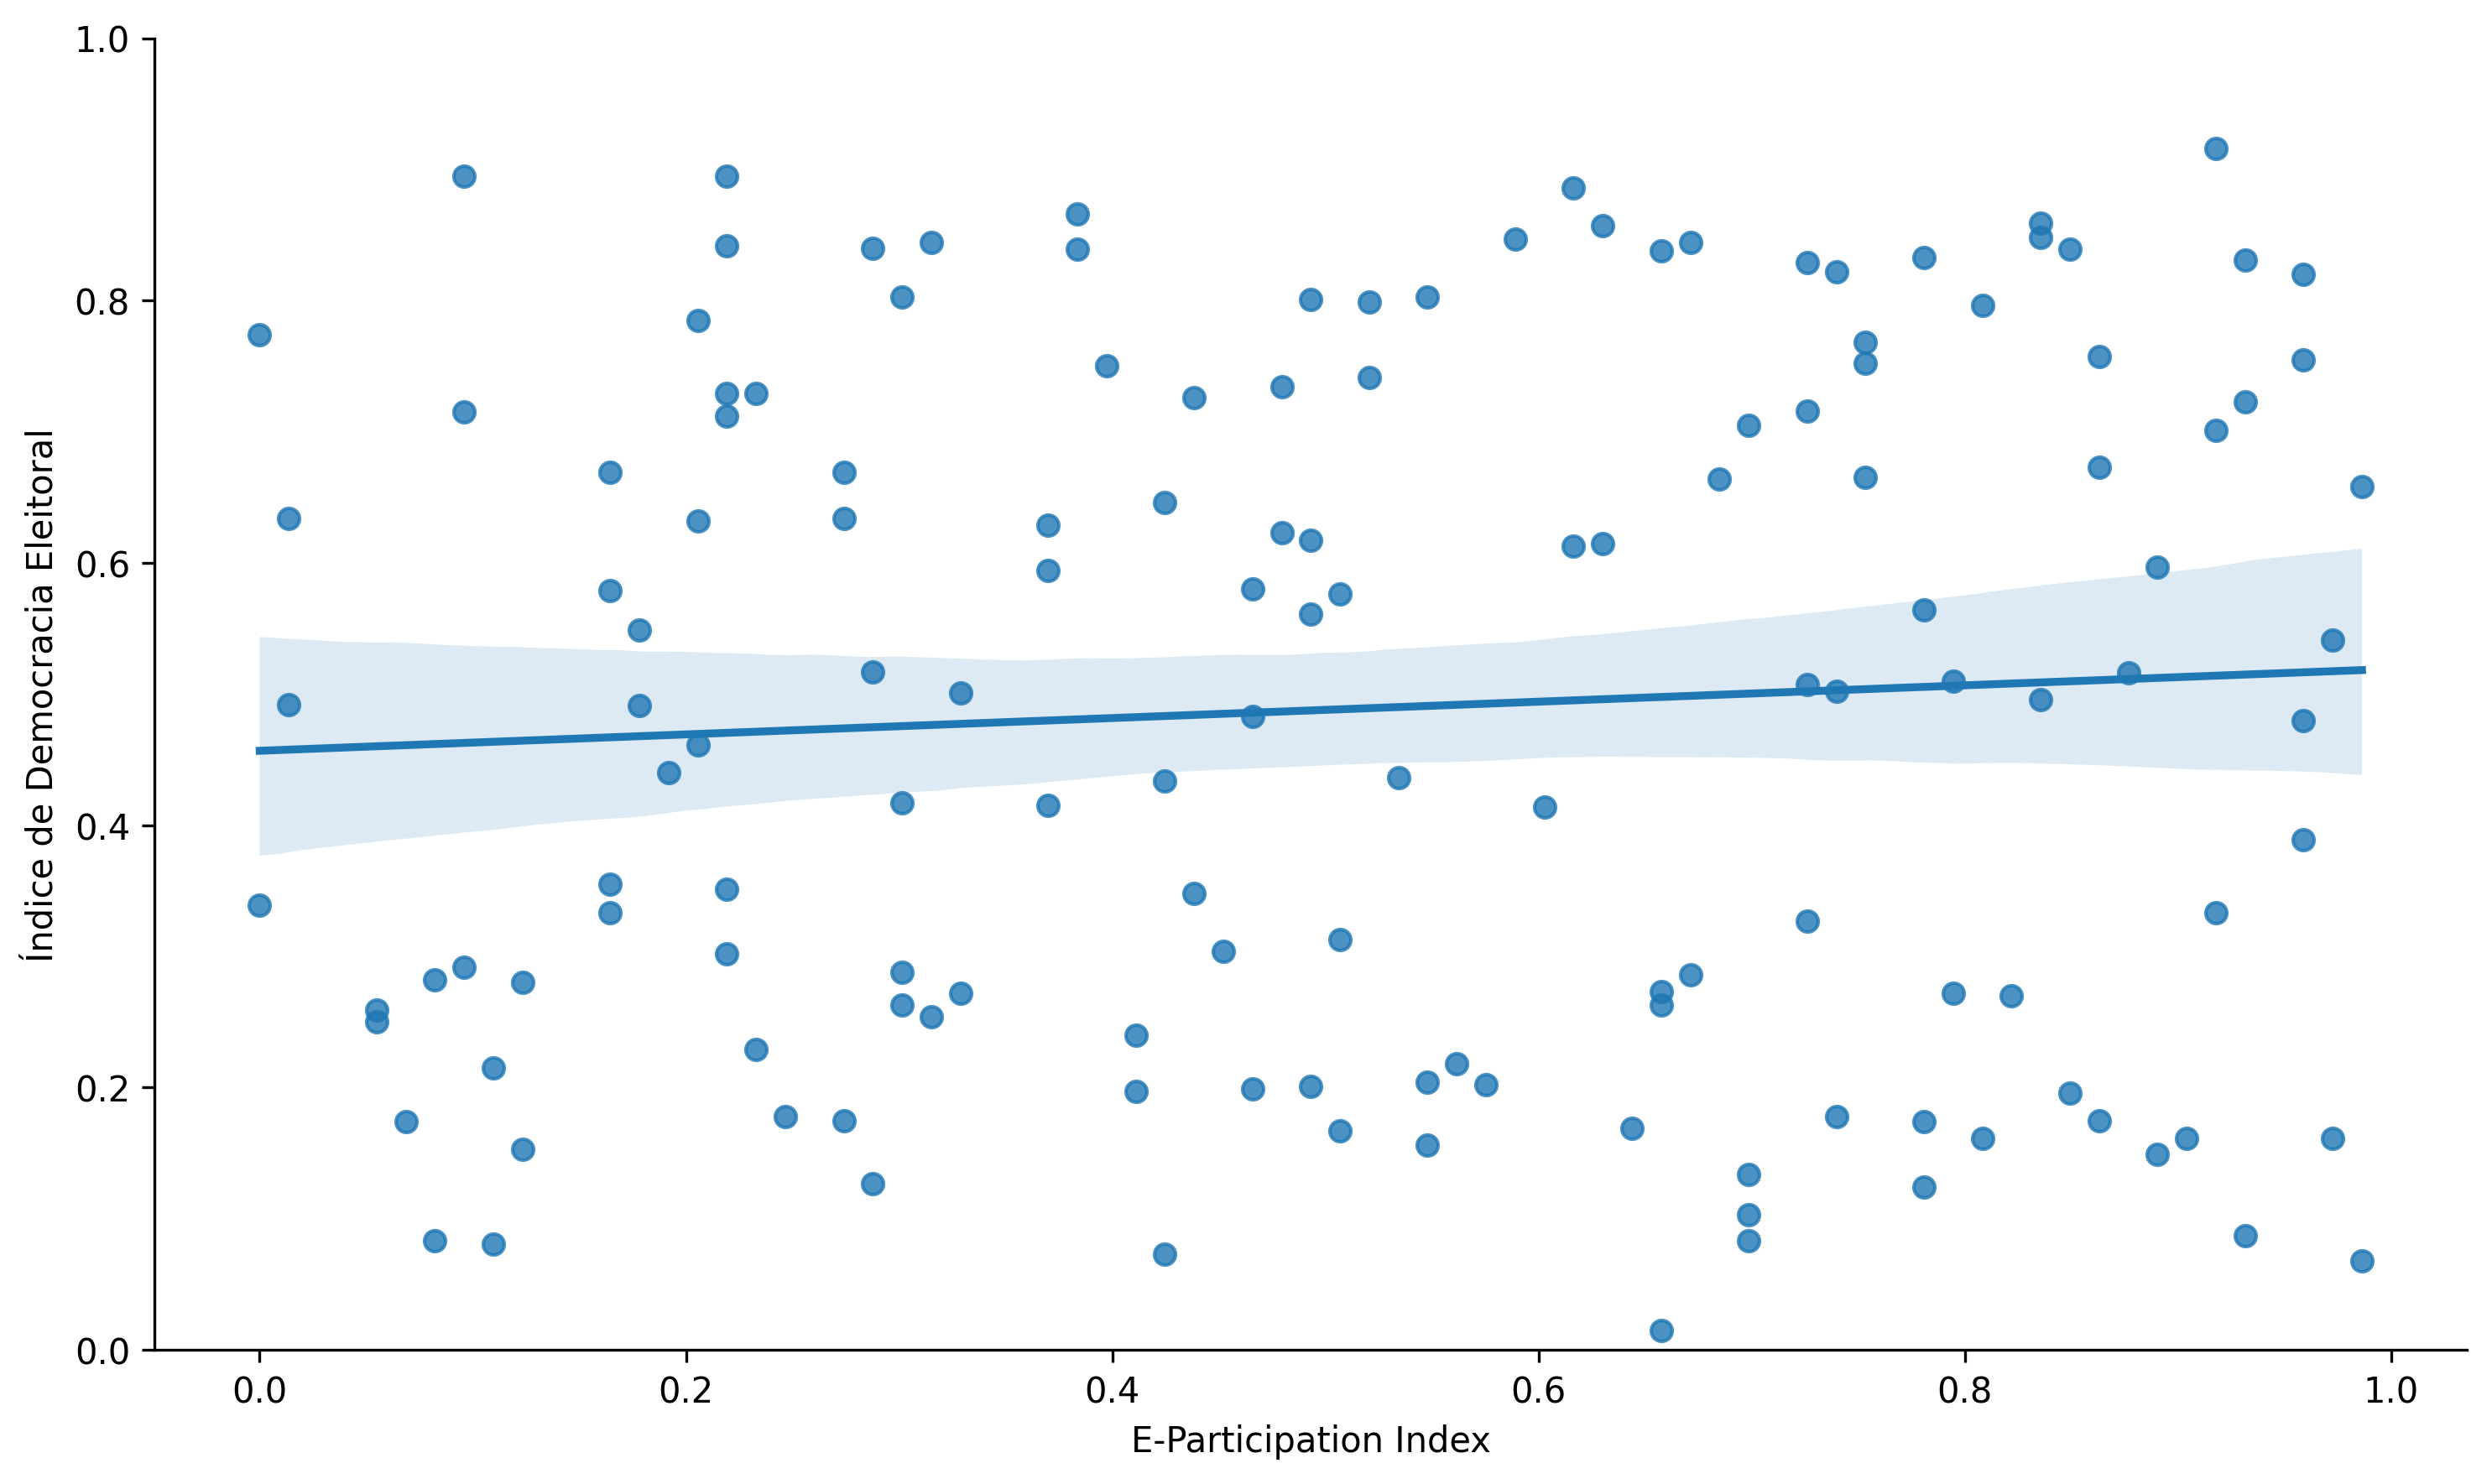
\includegraphics[width=1\linewidth]{figuras/egdi/dispersao_epart_indicedemocracia}
	\label{fig:dispersao_epart_indicedemocracia}
	\footnotesize{Fonte:baseado em \cite{ONU_EGDI_mapa} e \cite{electoral_democracy_index}}
\end{figure}

Para compreender melhor o diagrama de dispersão, foi usado o coeficiente de correlação de Spearman. A sua escolha foi motivada pela grande presença de pontos extremos. O coeficiente de correlação encontrada foi 0.05. Os índice de democracia eleitoral e o \textbf{E-Participation Index} são variáveis independentes.

\subsubsection{E-Government Development Index e gastos governamentais, percentagem do PIB}

\begin{figure}[H]
	\centering
	\caption{Diagrama de Dispensao: E-Government Development Index e gastos governamentais, percentagem do PIB}
	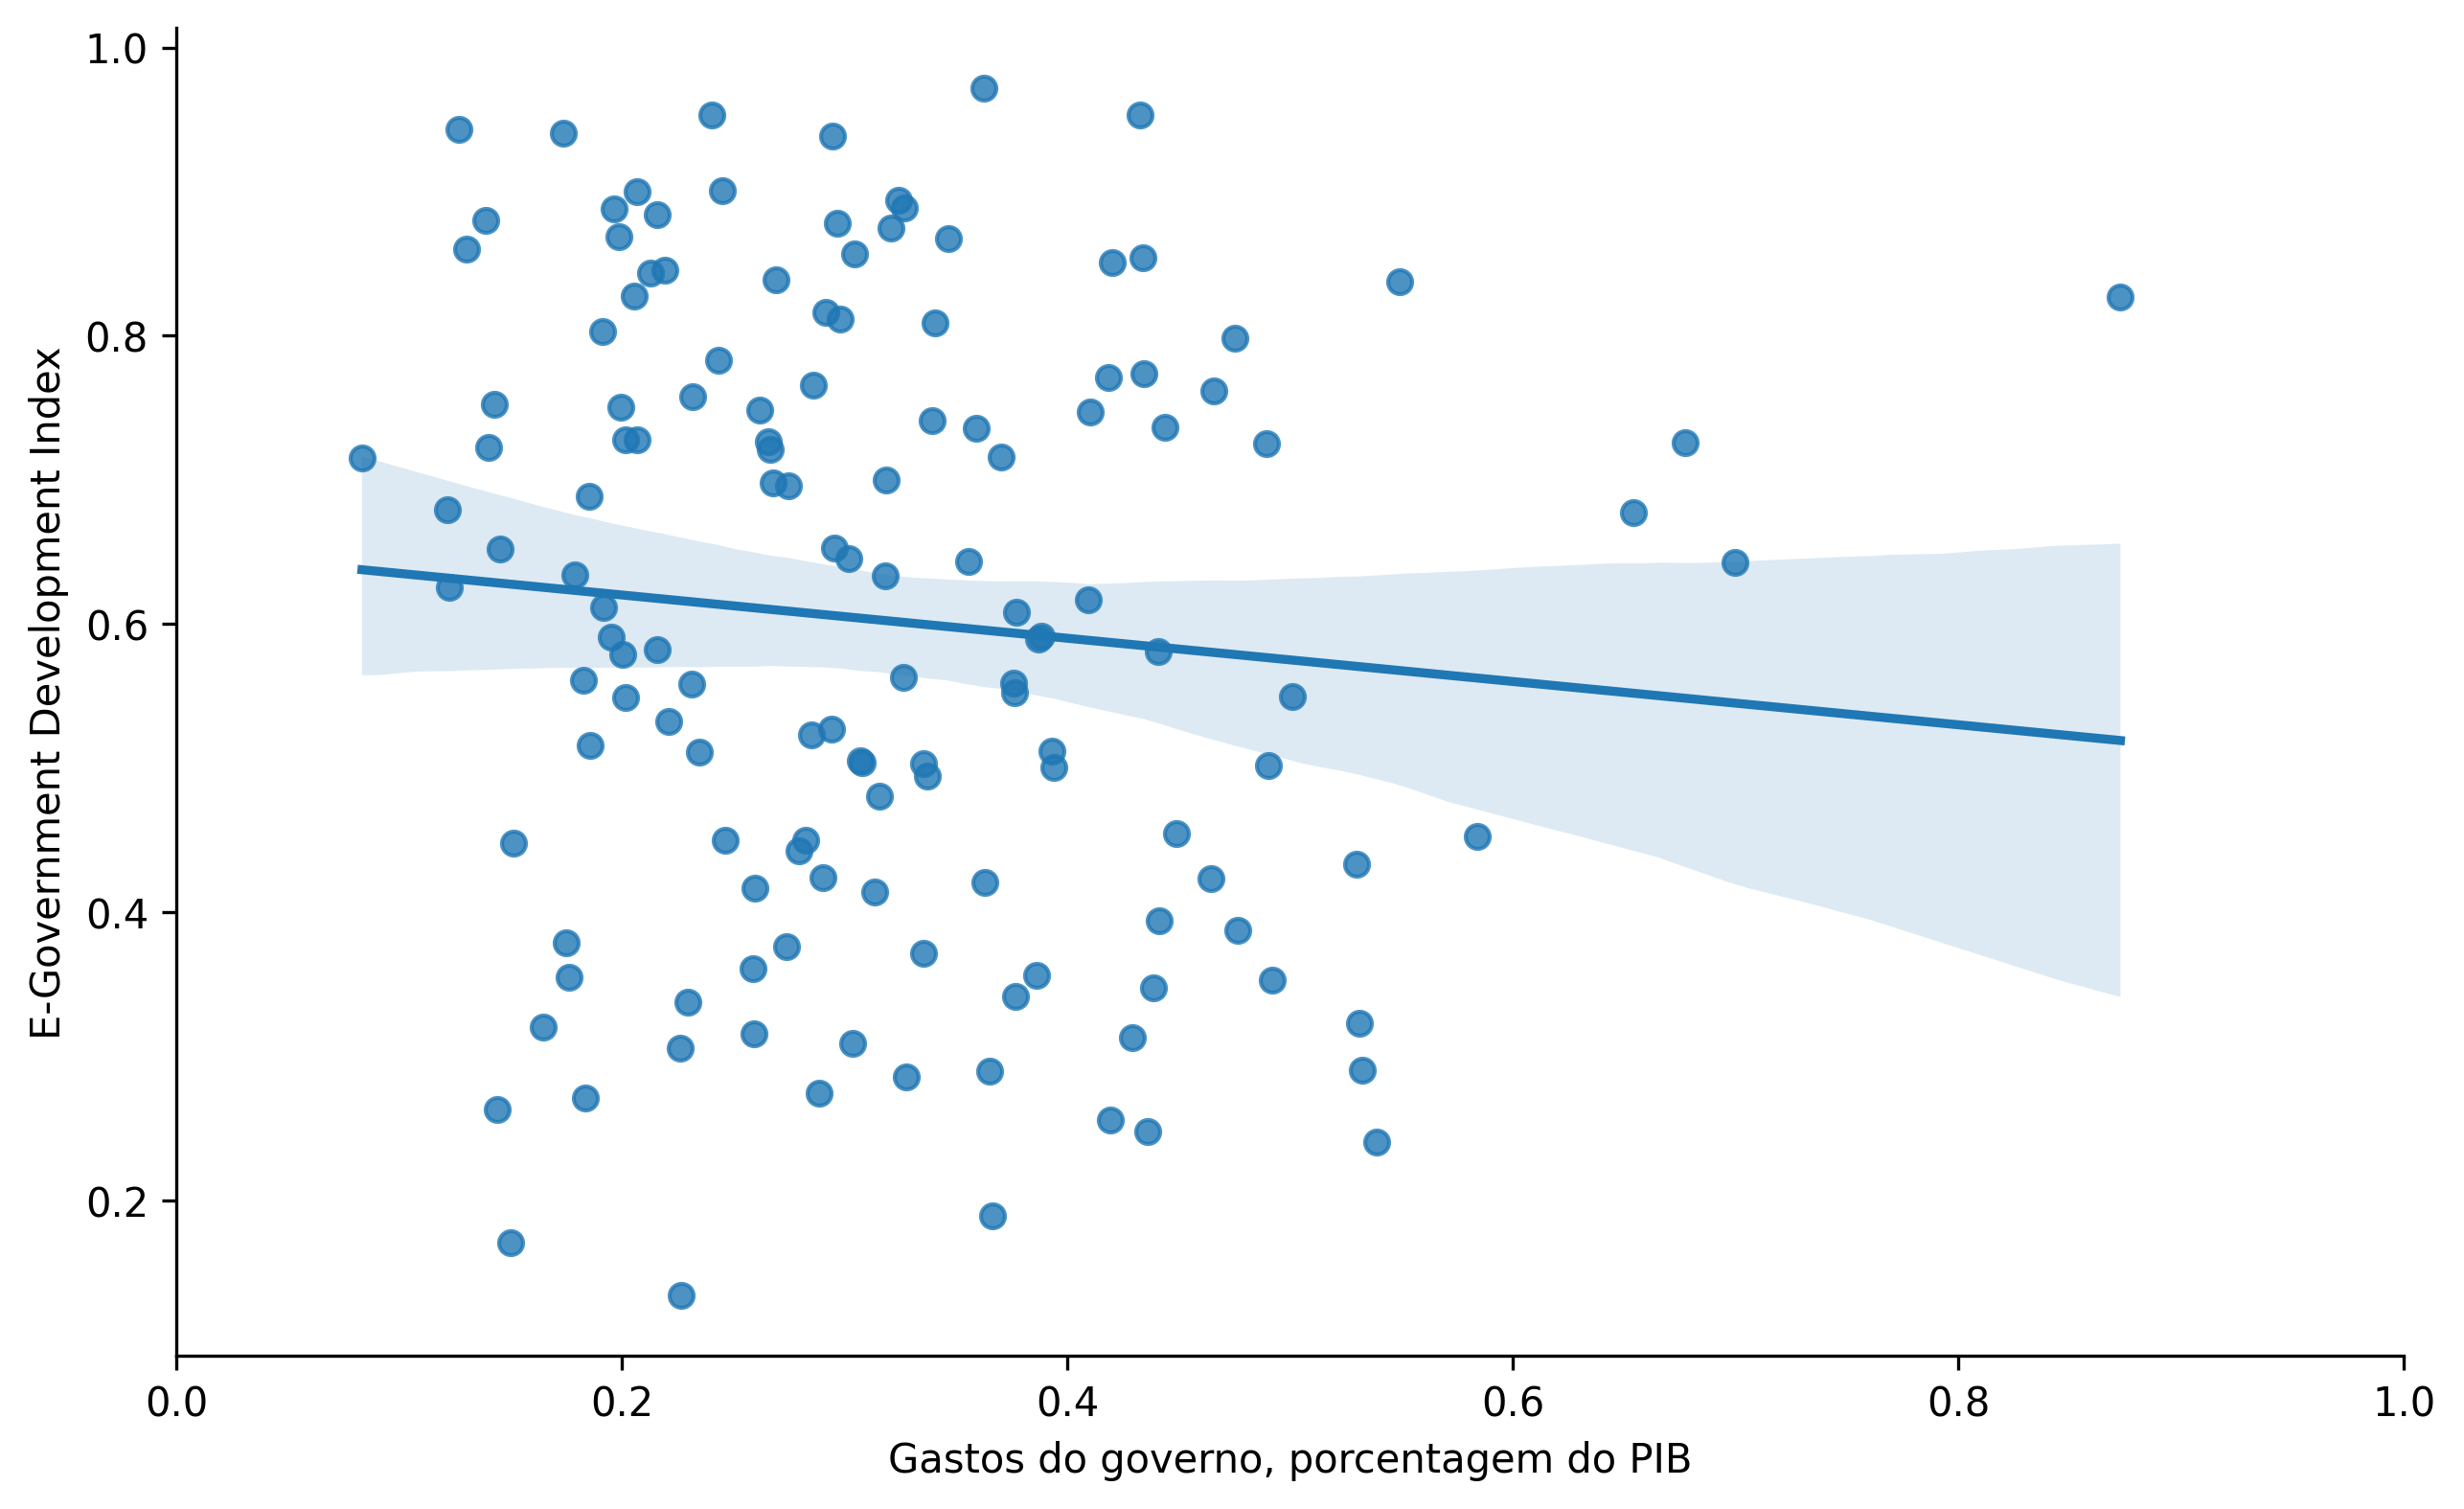
\includegraphics[width=1\linewidth]{figuras/egdi/dispersao_egov_govexpenditure}
	\label{fig:dispersao_egov_govexpenditure}
	\footnotesize{Fonte:baseado em \cite{ONU_EGDI_mapa} e \cite{FMI_gov_expenditure}}
\end{figure}

Para compreender melhor o diagrama de dispersão, foi usado o coeficiente de correlação de Spearman. A sua escolha foi motivada pela grande presença de pontos extremos. O coeficiente de correlação encontrada foi -0.13. O \textbf{E-Government Development Index} e os gastos governamentais são variáveis independentes.

\subsubsection{E-Participation Index e gastos governamentais, percentagem do PIB}

\begin{figure}[H]
	\centering
	\caption{Diagrama de Dispensao: E-Participation Index e gastos governamentais, percentagem do PIB}
	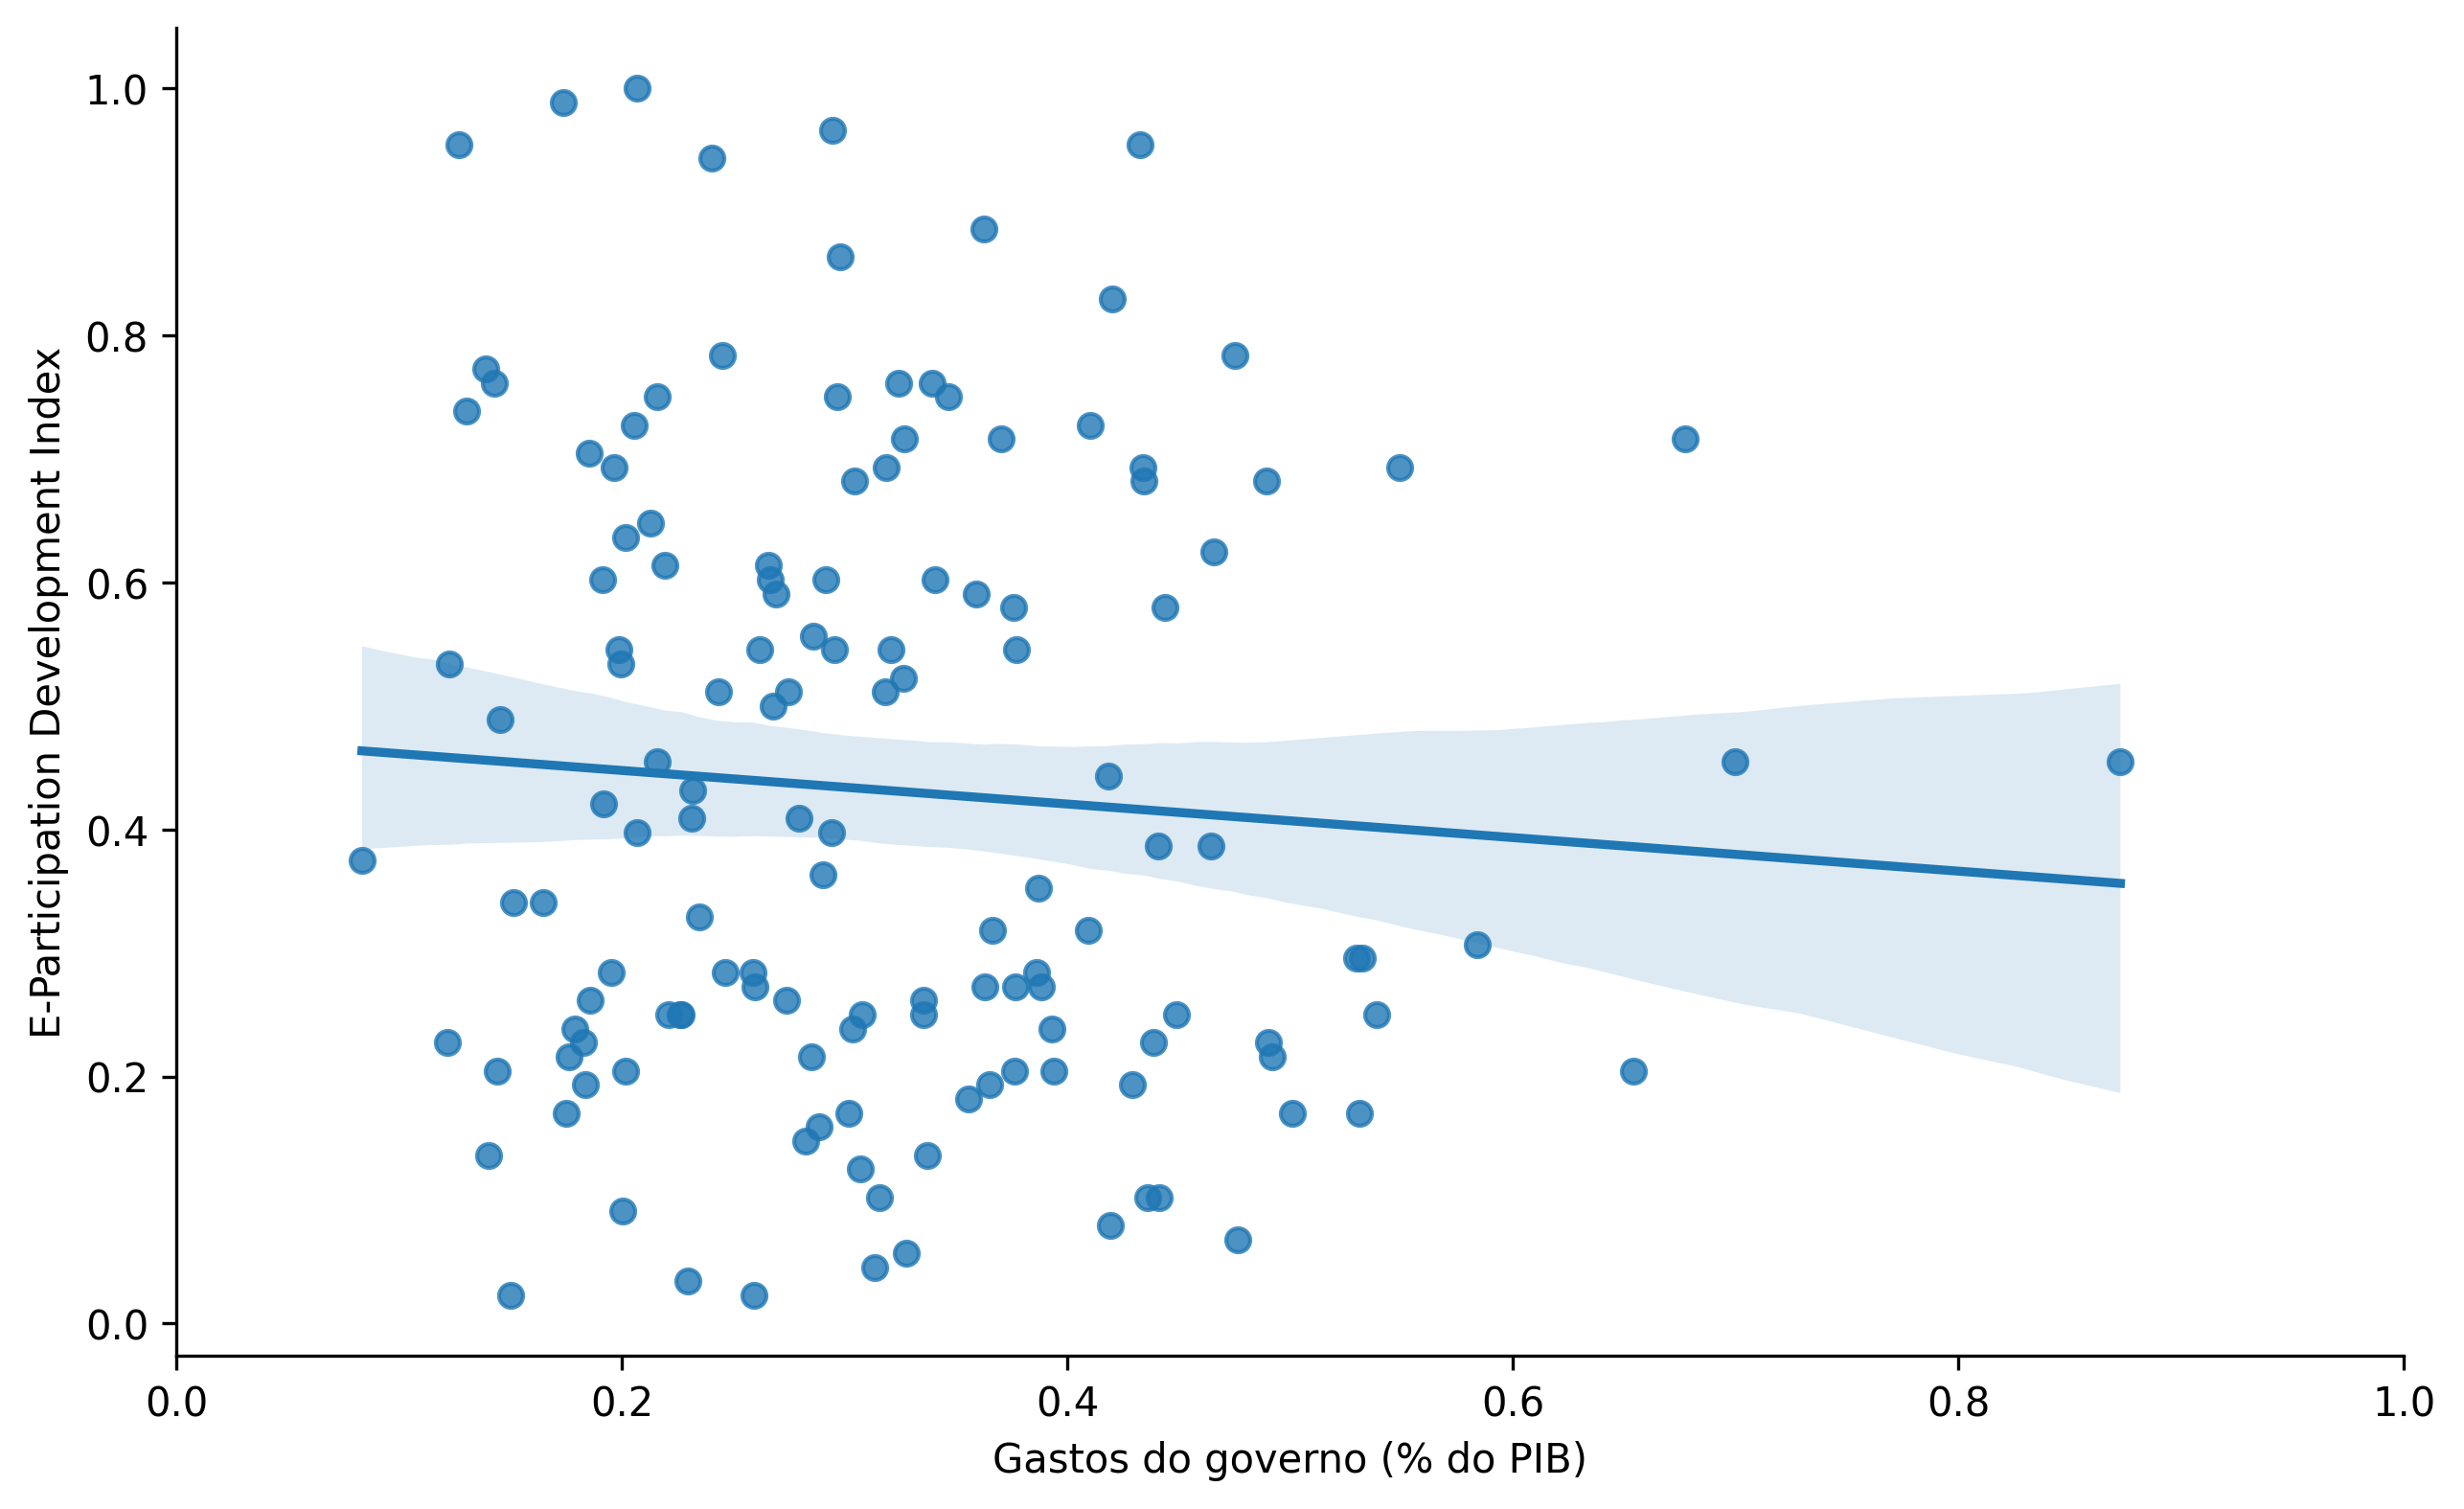
\includegraphics[width=1\linewidth]{figuras/egdi/dispersao_epart_govexpenditure}
	\label{fig:dispersao_epart_govexpenditure}
	\footnotesize{Fonte:baseado em \cite{ONU_EGDI_mapa} e \cite{FMI_gov_expenditure}}
\end{figure}

Para compreender melhor o diagrama de dispersão, foi usado o coeficiente de correlação de Spearman. A sua escolha foi motivada pela grande presença de pontos extremos. O coeficiente de correlação encontrada foi -0.07. O \textbf{E-Government Participation Index} e os gastos governamentais são variáveis independentes.

\subsection{Análise granular com os componentes do EGDI}

\subsubsection{PIB \textit{per capita} PPC}

\subsubsection{PIB \textit{per capita} PPC}

\subsubsection{PIB \textit{per capita} PPC}

\subsubsection{índice de democracia eleitoral}

\subsubsection{índice de democracia eleitoral}

\subsubsection{índice de democracia eleitoral}

\subsubsection{gastos governamentais, percentagem do PIB}

\subsubsection{gastos governamentais, percentagem do PIB}

\subsubsection{gastos governamentais, percentagem do PIB}

\section{Trabalhos de outros autores}

\cite{alisherovna2021whether} chegou a uma conclusão similar na figura \ref{fig:usmanova_egdi_gdp} a da figura \ref{fig:dispensao_egov_pib}, porém o autor adotou a taxa de crescimento do PIB ao invés do PIB \textit{per capita} PPC.

\begin{figure}[H]
	\centering
	\caption{Como os países se posicionam em relação ao EGDI de acordo com sua taxa de crescimento do PIB}
	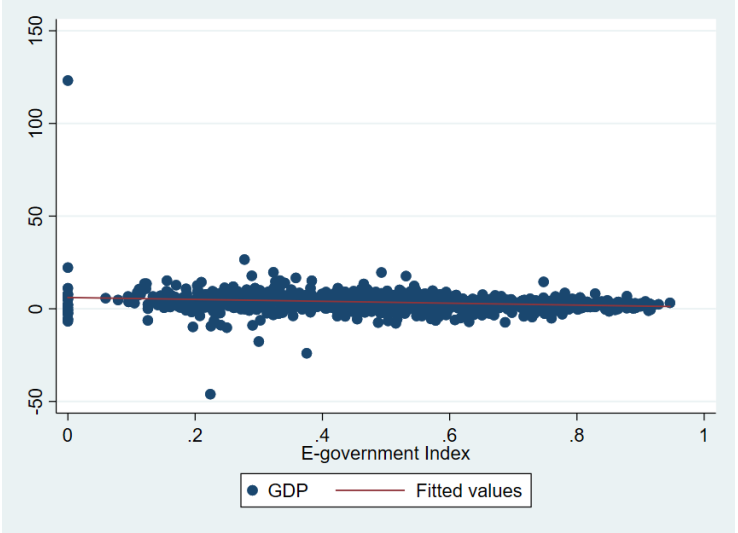
\includegraphics[width=1\linewidth]{figuras/egdi/usmanova_egdi_gdp}
	\label{fig:usmanova_egdi_gdp}
	\footnotesize{Fonte: \cite{alisherovna2021whether}}
\end{figure}

Embora a figura \ref{fig:usmanova_egdi_gdp} mostre menos pontos extremos do que a figura \ref{fig:dispensao_egov_pib}, percebe com o PIB, seja \textit{per capita} PPC ou sua taxa de crescimento tem forte correlação com o EGDI. 

Outros autores destacaram a importância do EGDI. \cite{kotenok2020government} concluem que o impacto do governo eletrônico pode impulsionar a inovação ou até mesmo ser um componente importante para entender como a economia é transformada devido à tecnologia. \cite{kumar2020cultural} descobriu que o desenvolvimento econômico, mensurado pelo PIB \textit{per capita}, significativamente e positivamente impulsio o EGDI. 

\cite{ziolo2022government} cita que na União Europe (até 2020), observou-se a correlação observada entre o nível de desenvolvimento do governo eletrônico e as áreas ambiental, social e econômica parece ser de grande importância. Essa correlação implica que a digitalização dos processos administrativos pode ter um impacto real no desenvolvimento sustentável, promovendo, assim, mudanças positivas em todas as suas três esferas.


\section{Indicadores de TIC de governo eletrônico}
\label{indicadores_tic_egov}

A ONU tem \href{https://publicadministration.un.org/egovkb/en-us/Data/ICT-in-government}{indicadores de TIC de governo eletrônico} como algo complementar ao EGDI. Os indicadores são, conforme \cite{ONU_ICT_in_government_indicators}:

\begin{itemize}
	\item Existência de estratégia nacional de governo eletrônico ou equivalente;
	\item Existência de identidade digital para acessar ou outra forma de autenticação requirida para poder acessar serviços online;
	\item Existência de um portal de compras governamentais.
\end{itemize}

Os resultados globais dos indicadores estão presentes nas figuras \ref{fig:national_government_strategy}, \ref{fig:national_identity} e \ref{fig:procurement_portal}.

\begin{figure}[H]
	\centering
	\caption{Indicador: Existência de estratégia nacional de governo eletrônico ou equivalente}
	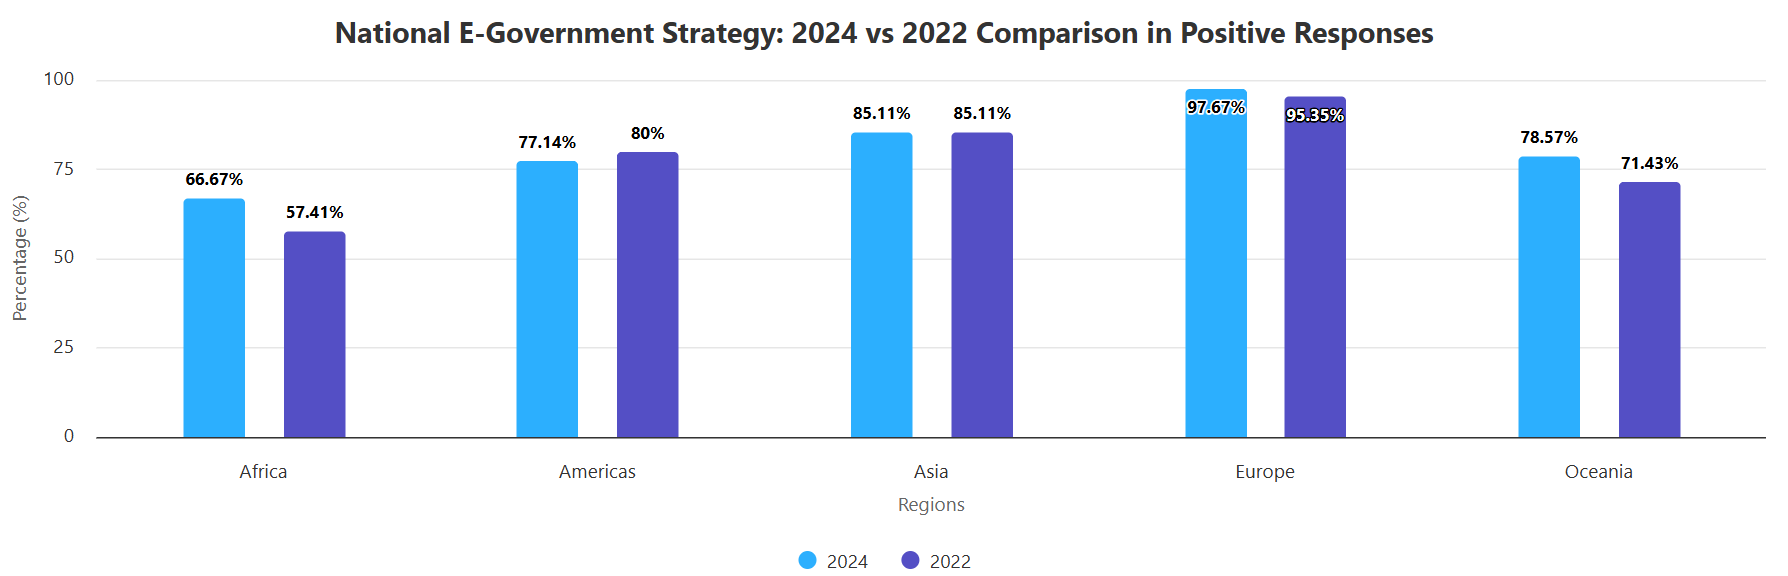
\includegraphics[width=1\linewidth]{figuras/ict_in_government/national_government_strategy}
	\label{fig:national_government_strategy}
	\footnotesize{Fonte: \cite{ONU_ICT_in_government_indicators}}
\end{figure}

\begin{figure}[H]
	\centering
	\caption{Indicador: Existência de identidade digital para acessar ou outra forma de autenticação requirida para poder acessar serviços online}
	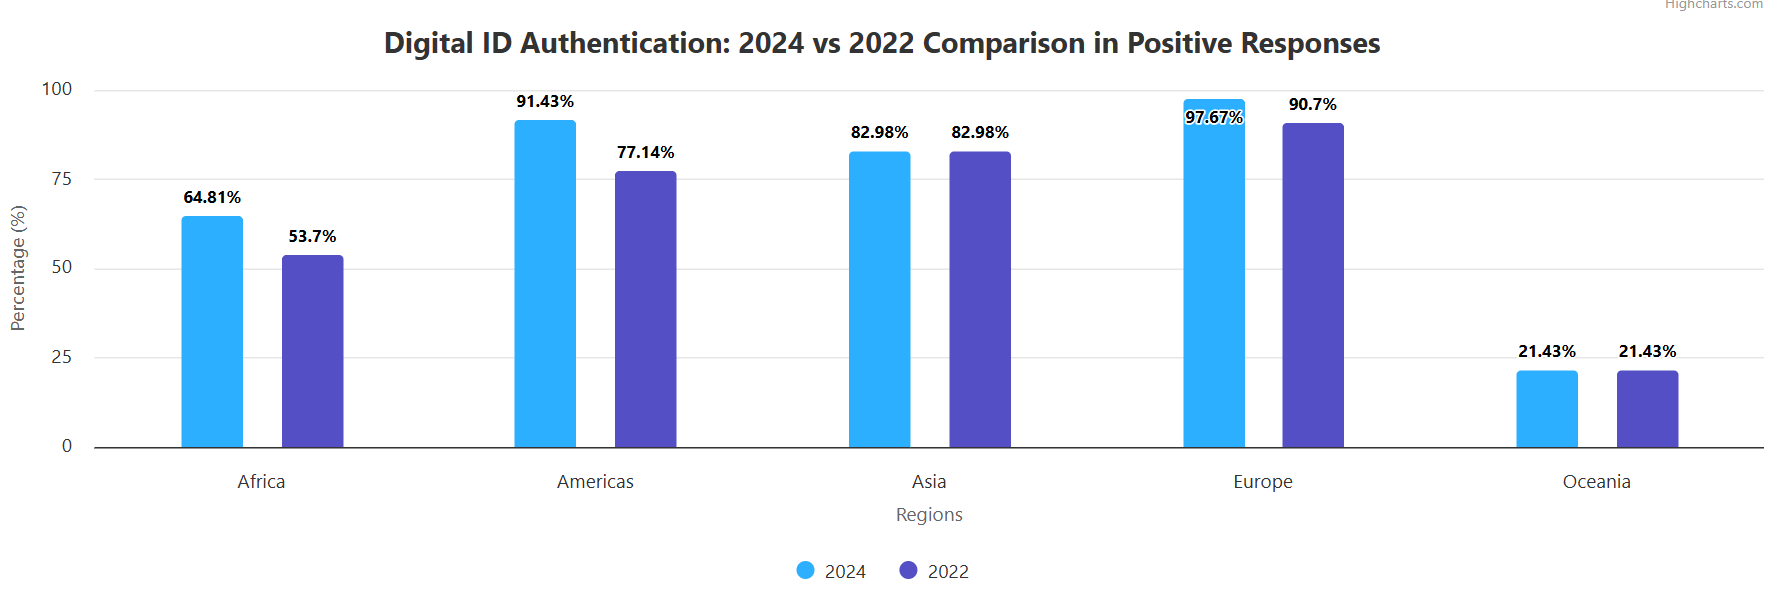
\includegraphics[width=1\linewidth]{figuras/ict_in_government/digital_identity}
	\label{fig:national_identity}
	\footnotesize{Fonte: \cite{ONU_ICT_in_government_indicators}}
\end{figure}

\begin{figure}[H]
	\centering
	\caption{Indicador: Existência de um portal de compras governamentais}
	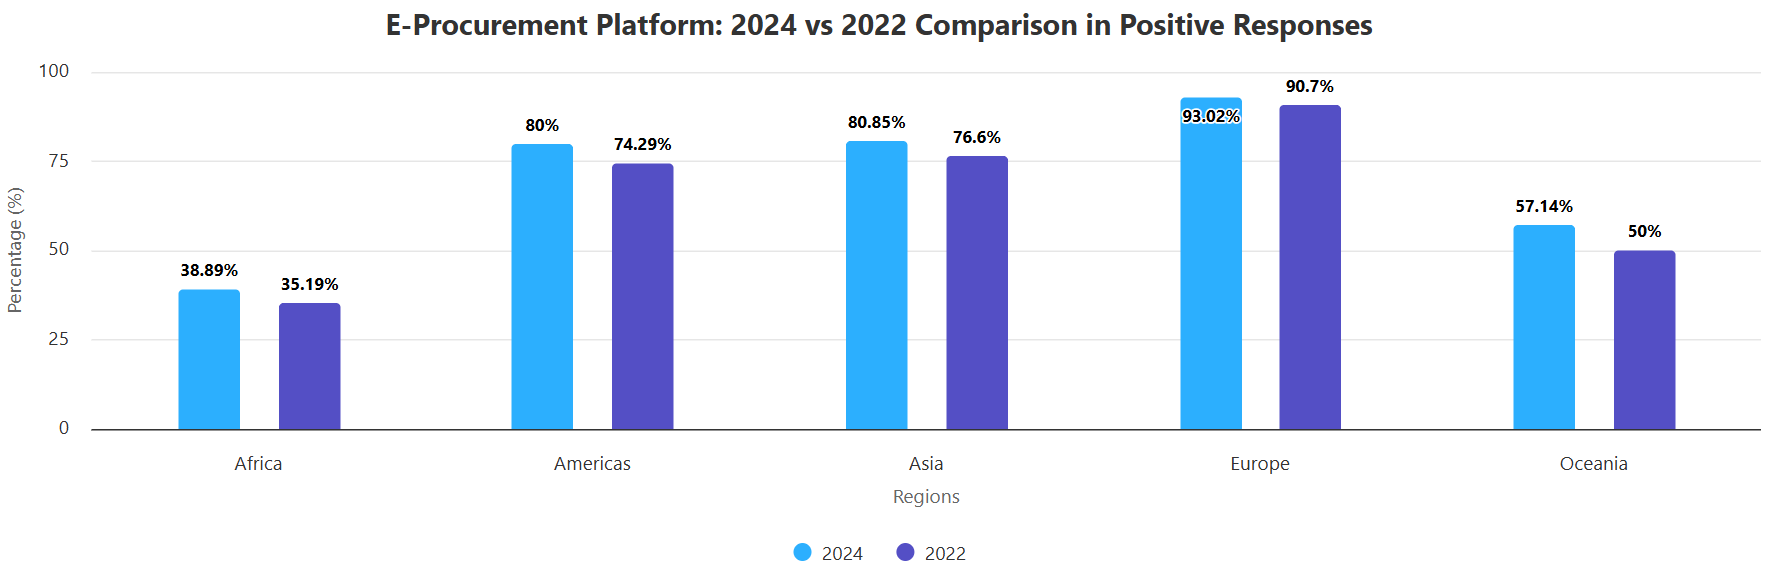
\includegraphics[width=1\linewidth]{figuras/ict_in_government/procurement_portal}
	\label{fig:procurement_portal}
	\footnotesize{Fonte: \cite{ONU_ICT_in_government_indicators}}
\end{figure}

Extraí-se das três figuras que a Europa foi o continente cujos mais respondem que têm seguem os indicadores, superando os 90\%. A Oceania foi o continente que menos implementou políticas de identidade digital para acesso a serviços online. África e Oceania tiveram um desempenho ruim na implementação de portais de compra governamentais. O continente americano apresentou bom desempenho nos três indicadores.

Como consequência da análise dos resultados presentes nas figuras \ref{fig:national_government_strategy}, \ref{fig:national_identity} e \ref{fig:procurement_portal}, buscou-se entender a seguinte situação registrada nos 2022 e 2024, anos em que os indicadores foram medidos: qual é a porcentagem de países que responderam nenhuma, uma, duas ou todas as perguntas. Elas usam sim ou não para confirmar a aplicação dos indicadores no país.

A resposta ao questionamento está presente na figura \ref{fig:indicators_answer}.

\begin{figure}[H]
	\centering
	\caption{Respostas positivas aos indicadores de TIC de governo eletrônico}
	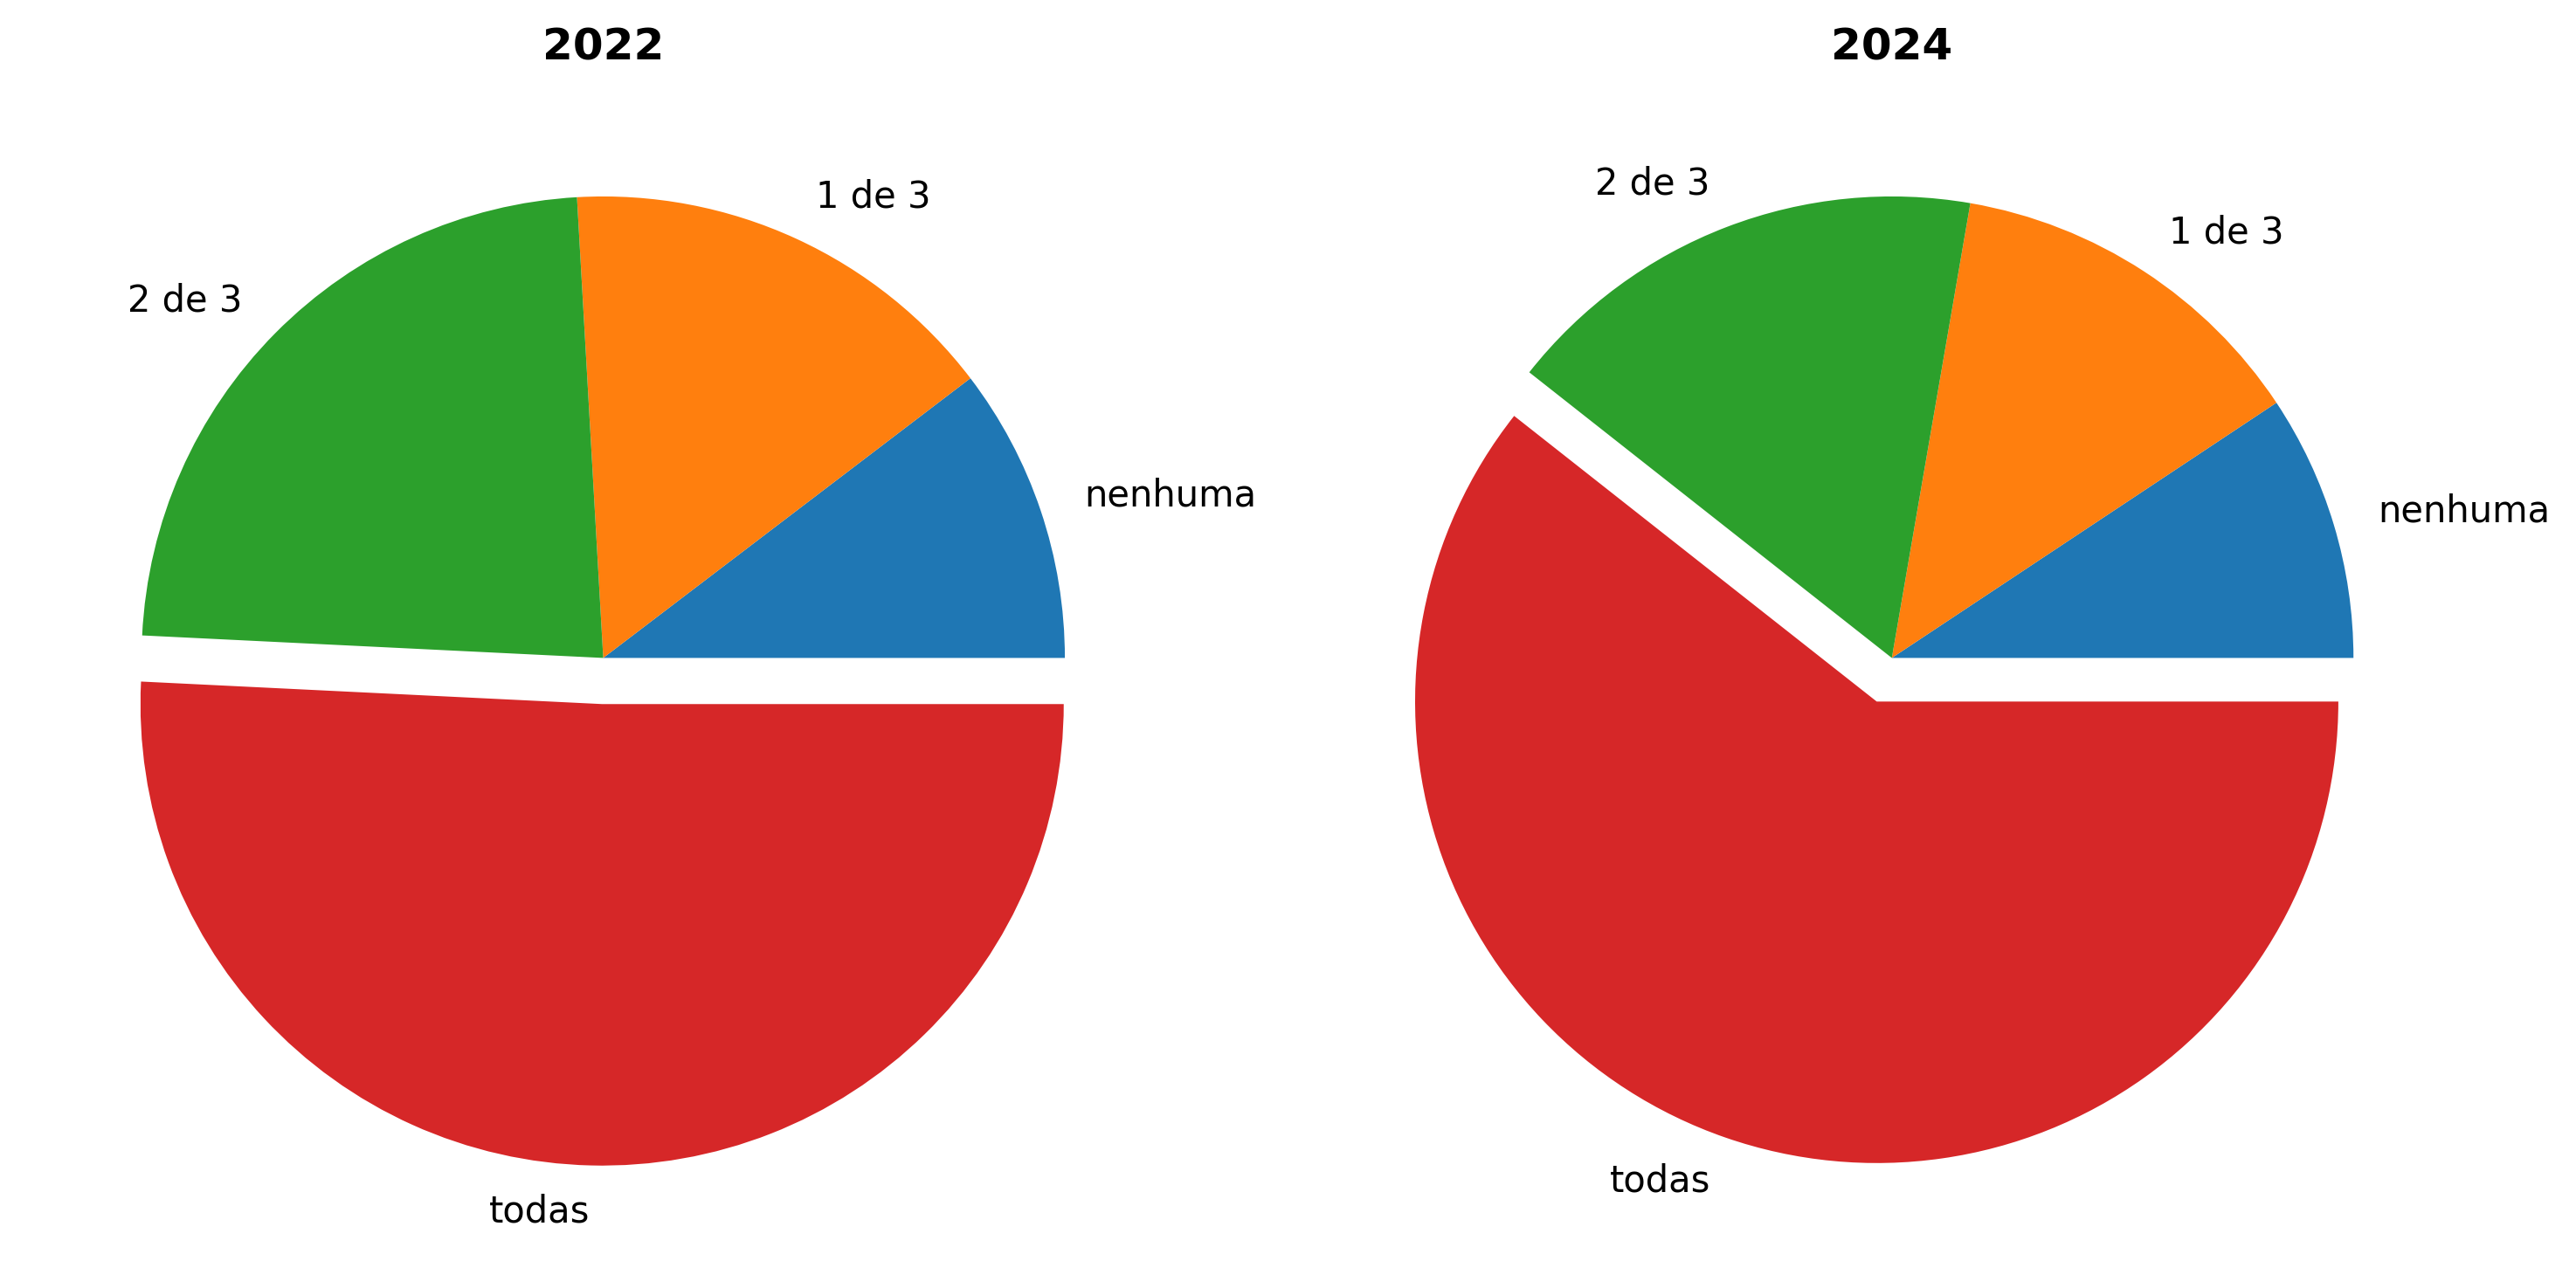
\includegraphics[width=1\linewidth]{figuras/ict_in_government/indicators_answer}
	\label{fig:indicators_answer}
	\footnotesize{Fonte: \cite{ONU_ICT_in_government_indicators}}
\end{figure}

Em 2022, metade dos países respondeu positivamente as três perguntas; em 2024, mais da metade. O Brasil faz parte desse grupo, tal como a Rússia e China. A mudança é creditada a redução do número de países que responderam positivamente 2 de 3 perguntas e passaram a responder as três positivamente. 

Além, disso a quantidade de países que responderam positivamente 1 de 3 perguntas e nenhuma se igualou em 2024, sendo os países que responderam 1 de 3 perguntas era maior do que os que responderam nenhuma.

\section{Coeficiente de correlação: indicadores de TIC de governo eletrônico comparados com outras variáveis}

Com base no parágrafo \ref{indicadores_tic_egov}, buscou-se entender se há correlação entre os indicadores de TIC de governo eletrônico e os PIB \textit{per capita} PPC e índice de democracia eleitoral.

\begin{figure}[H]
	\centering
	\caption{Diagrama de Dispersão: indicadores de TIC de governo eletrônico e PIB \textit{per capita} PPC}
	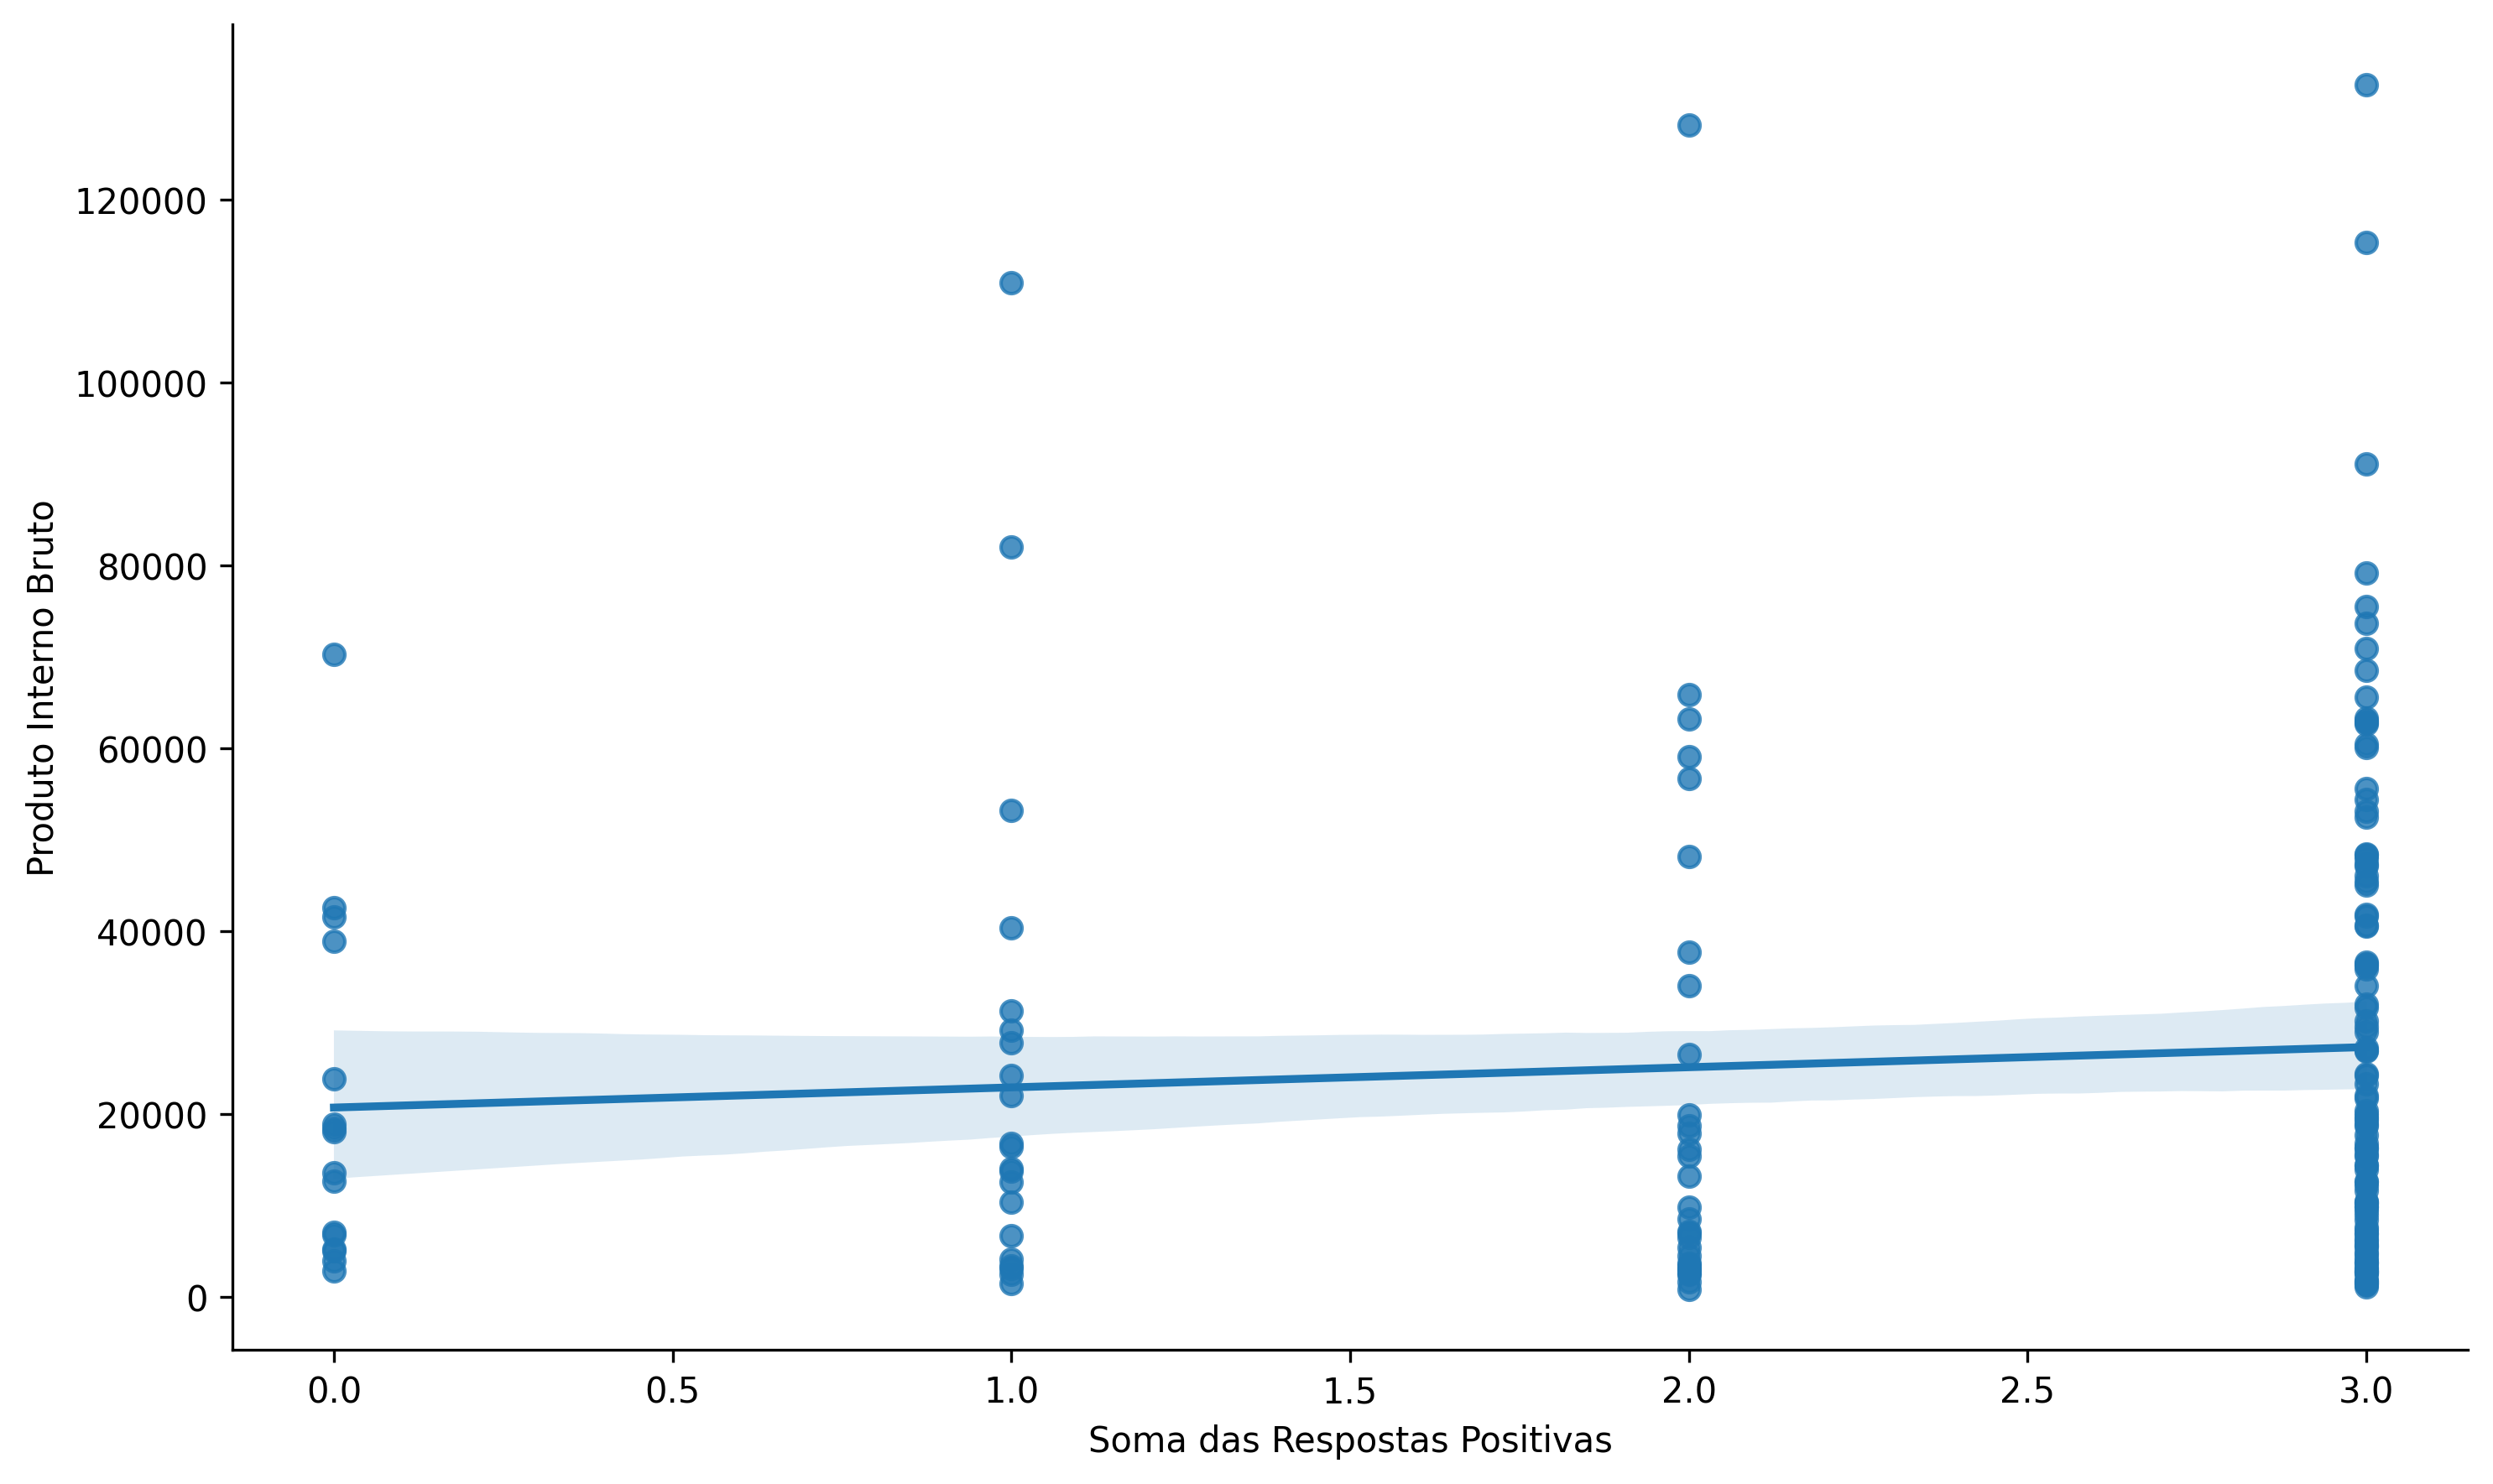
\includegraphics[width=1\linewidth]{figuras/ict_in_government/dispersao_ticegov_pib}
	\label{fig:dispersao_ticegov_pib}
	\footnotesize{Fonte: baseado em \cite{WB_pib_per_capita_países} e \cite{ONU_ICT_in_government_indicators}}
\end{figure}

\begin{figure}[H]
	\centering
	\caption{Diagrama de Dispersão: indicadores de TIC de governo eletrônico e índice de democracia eleitoral}
	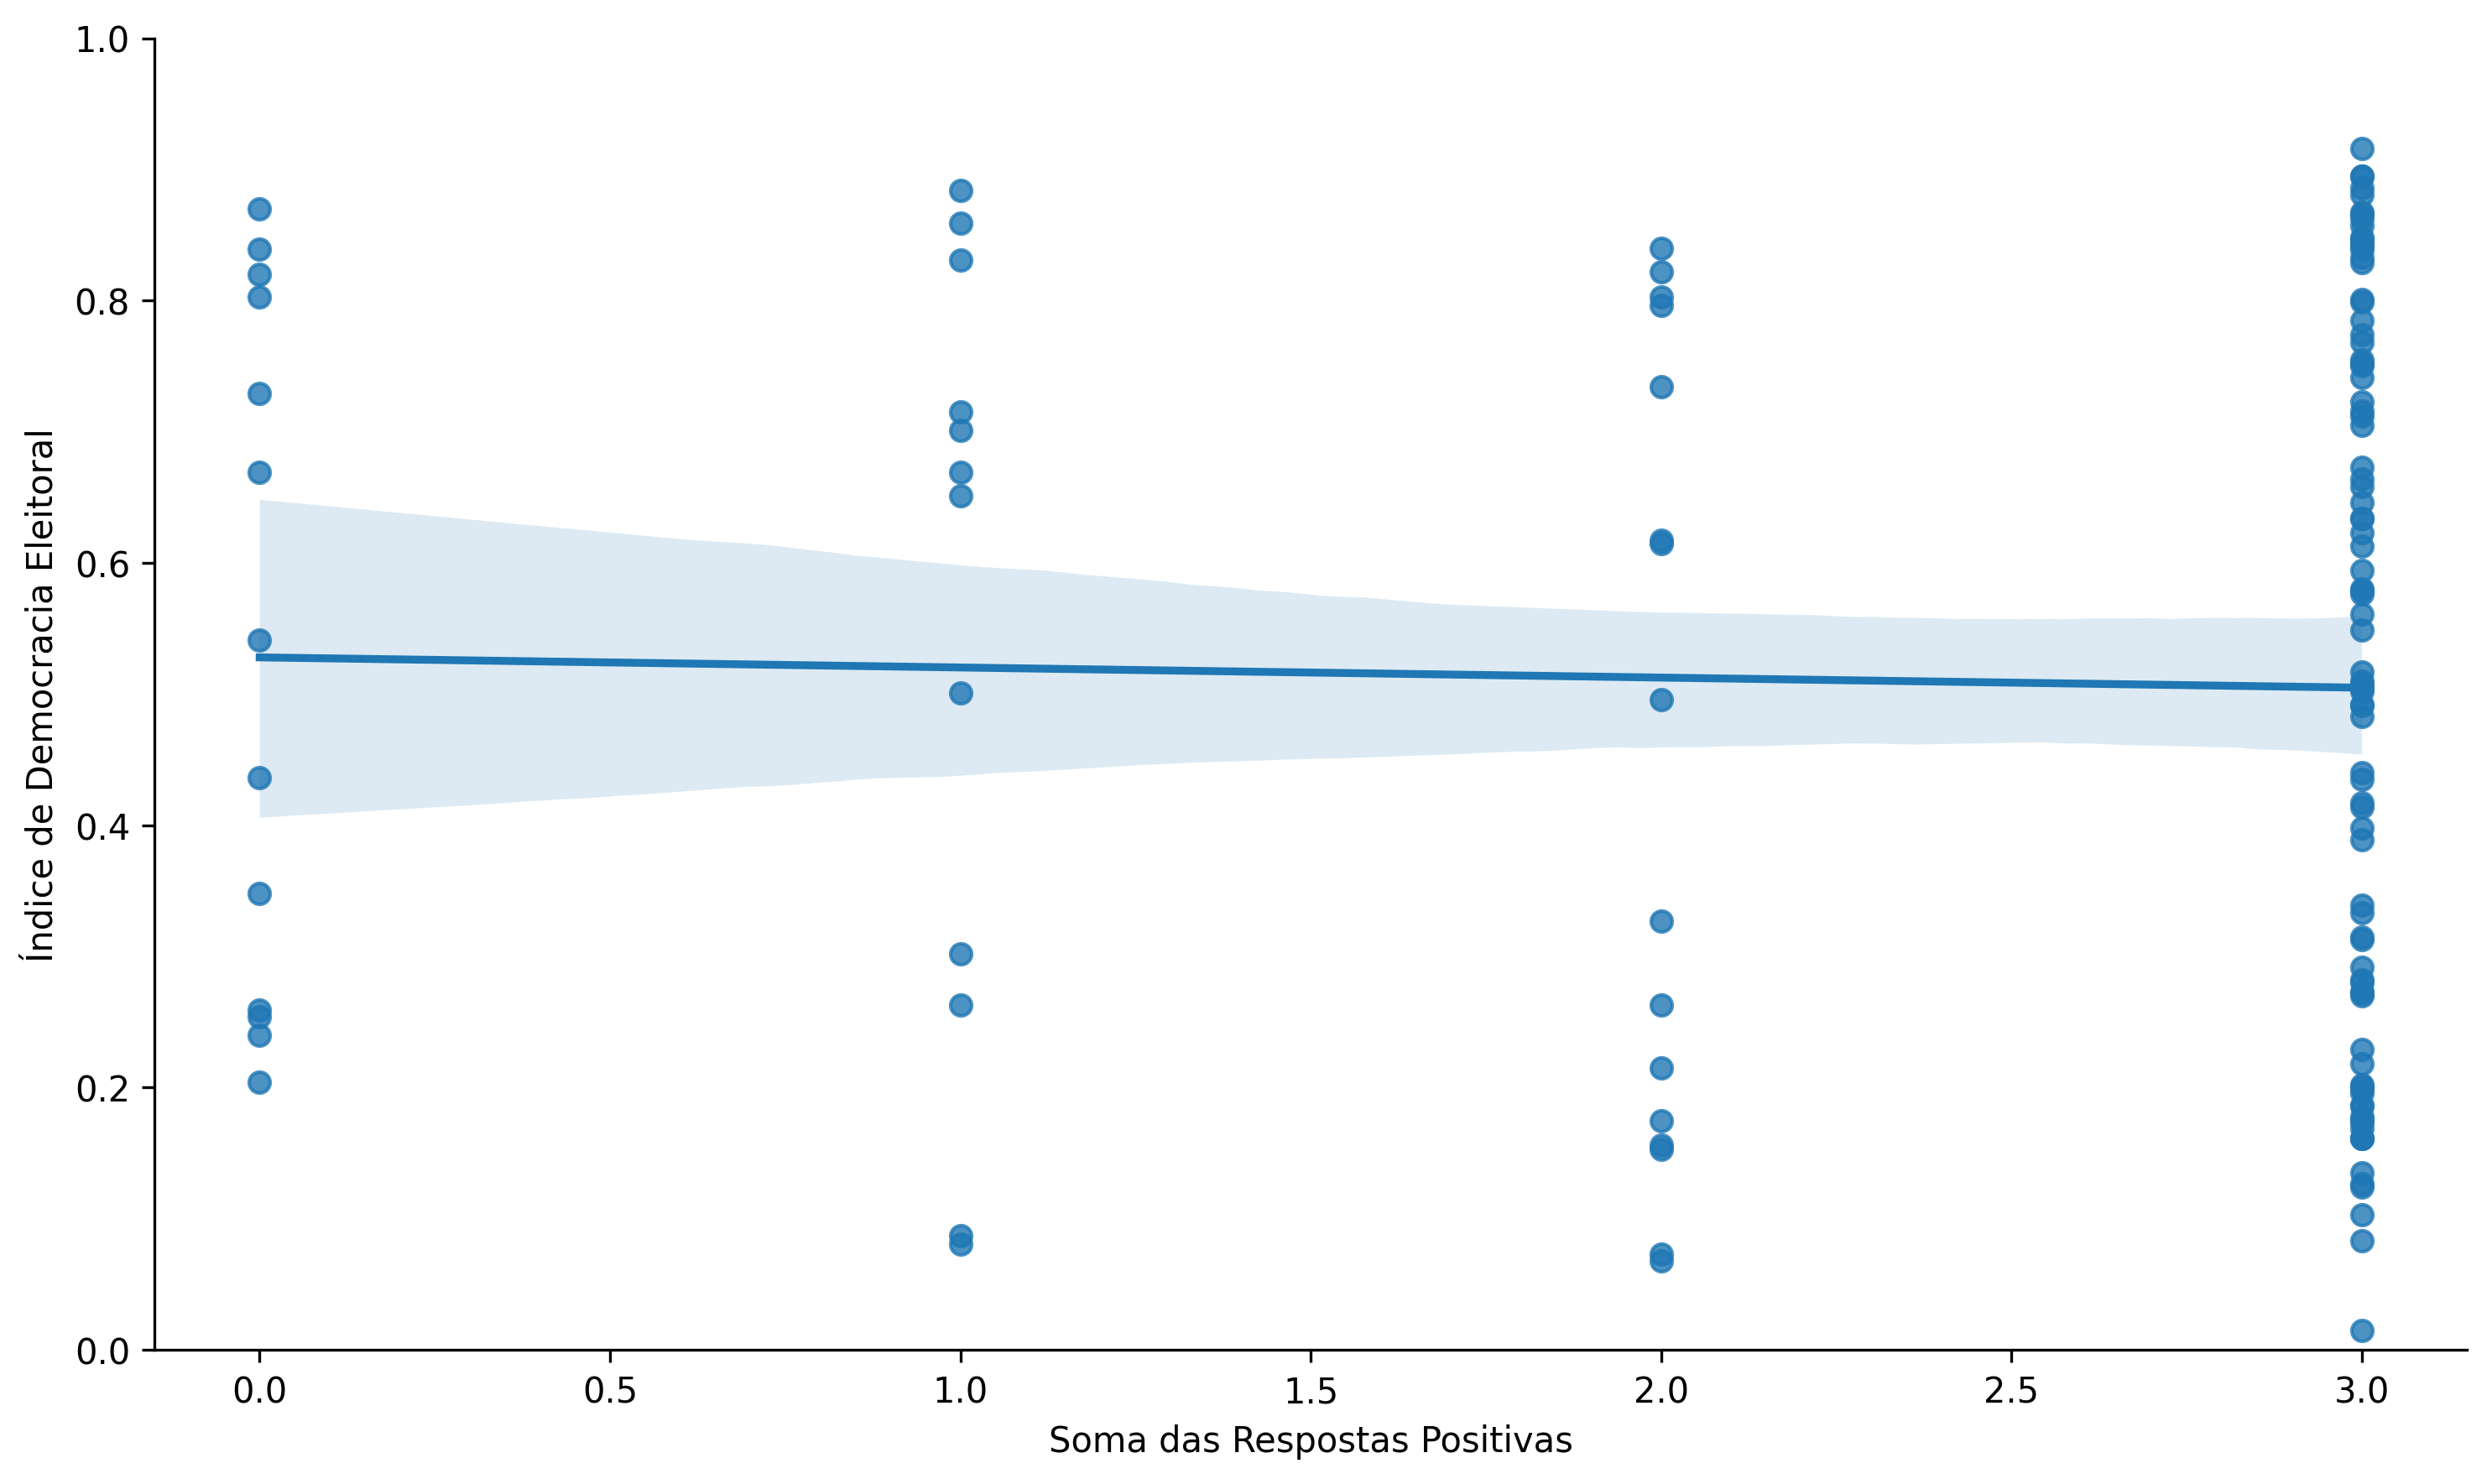
\includegraphics[width=1\linewidth]{figuras/ict_in_government/dispersao_ticegov_indicedemocracia}
	\label{fig:dispersao_ticegov_indicedemocracia}
	\footnotesize{Fonte: baseado em \cite{electoral_democracy_index} e \cite{ONU_ICT_in_government_indicators}}
\end{figure}

Como os diagramas de dispersão presentes nas figuras \ref{fig:dispersao_ticegov_pib} e \ref{fig:dispersao_ticegov_indicedemocracia}  apresentaram grande dispersão em relação à tendência, optou-se pelo uso do coeficiente de correlação de Spearman. A alta dispersão em relação à tendência é um indicativo de um coeficiente de correlação neutro ou baixo. Os coeficientes de correlação (0.1 e -0.0051) indicam que os indicadores de TIC de governo eletrônico não são afetados pelo PIB per capita PPC e pelo índice de democracia eleitoral, e vice-versa.

Outra análise feita foi a comparação entre os indicadores de TIC de governo eletrônico e os gastos governamentais.

\begin{figure}[H]
	\centering
	\caption{Diagrama de Dispersão: indicadores de TIC de governo eletrônico e gastos governamentais, percentagem do PIB}
	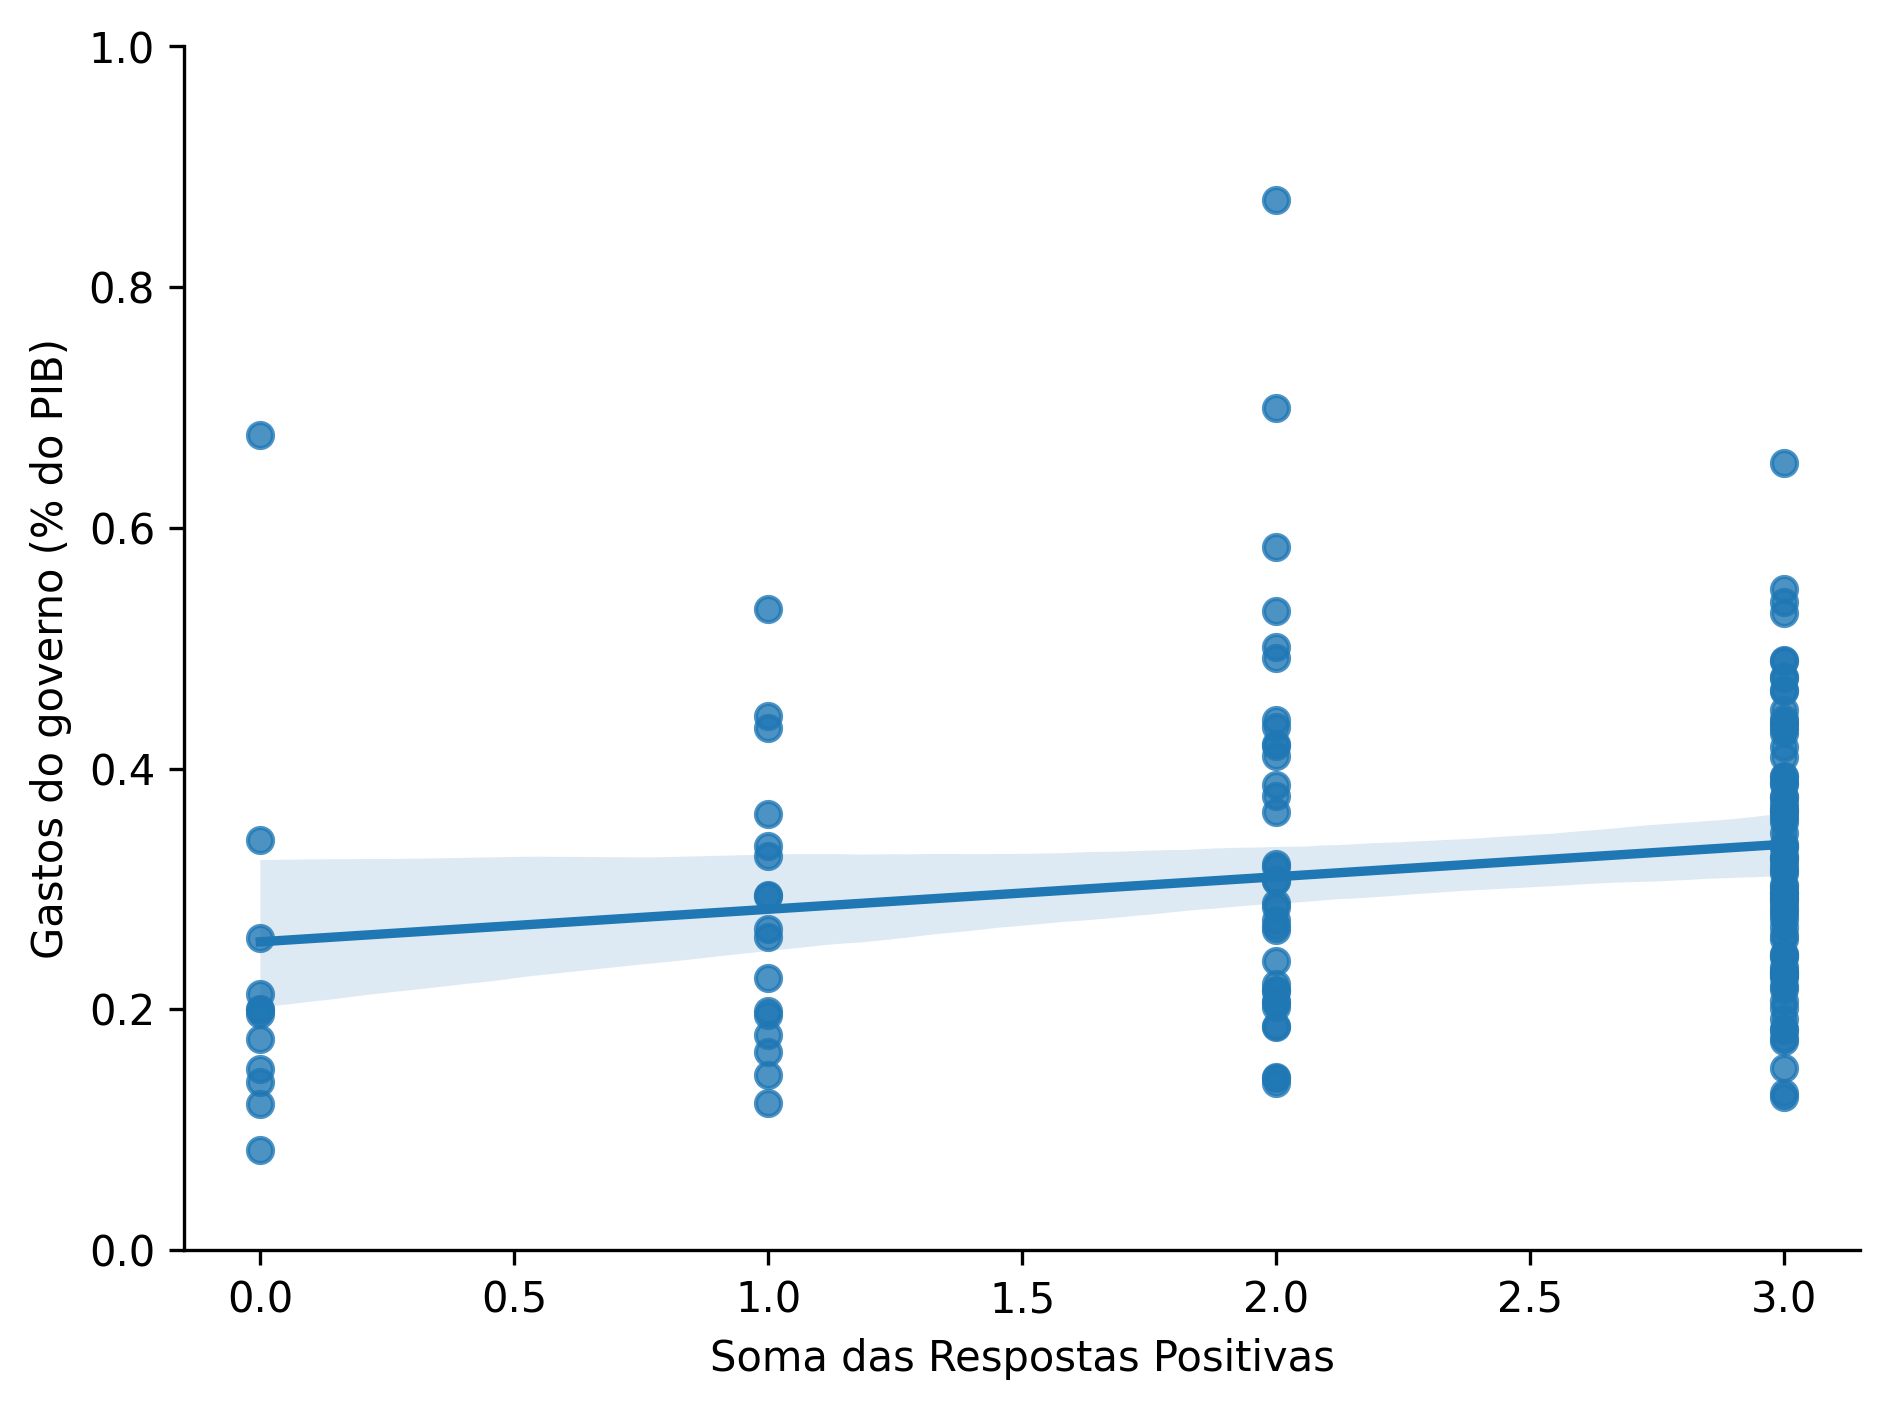
\includegraphics[width=1\linewidth]{figuras/egdi/dispersao_ticegov_govexpenditure}
	\label{fig:dispersao_ticegov_govexpenditure}
	\footnotesize{Fonte: baseado em \cite{FMI_gov_expenditure} e \cite{ONU_ICT_in_government_indicators}}
\end{figure}

Para compreender melhor o diagrama de dispersão, foi usado o coeficiente de correlação de Spearman. A sua escolha foi motivada pela grande presença de pontos extremos. O coeficiente de correlação encontrada foi 0.23. O referido coeficiente indica uma correlação positiva muito fraca entre os gastos do governo e a soma das respostas positivas. 


\section{EGDI do Brasil}

A figura \ref{fig:lineplot_egdi_brasil} mostra evolução do EGDI do Brasil desde 2003-2005 e 2008-2024 (bianualmente).

\begin{figure}[H]
	\centering
	\caption{Evolução do EGDI do Brasil (2003-2005, 2008-2024 bianualmente)}
	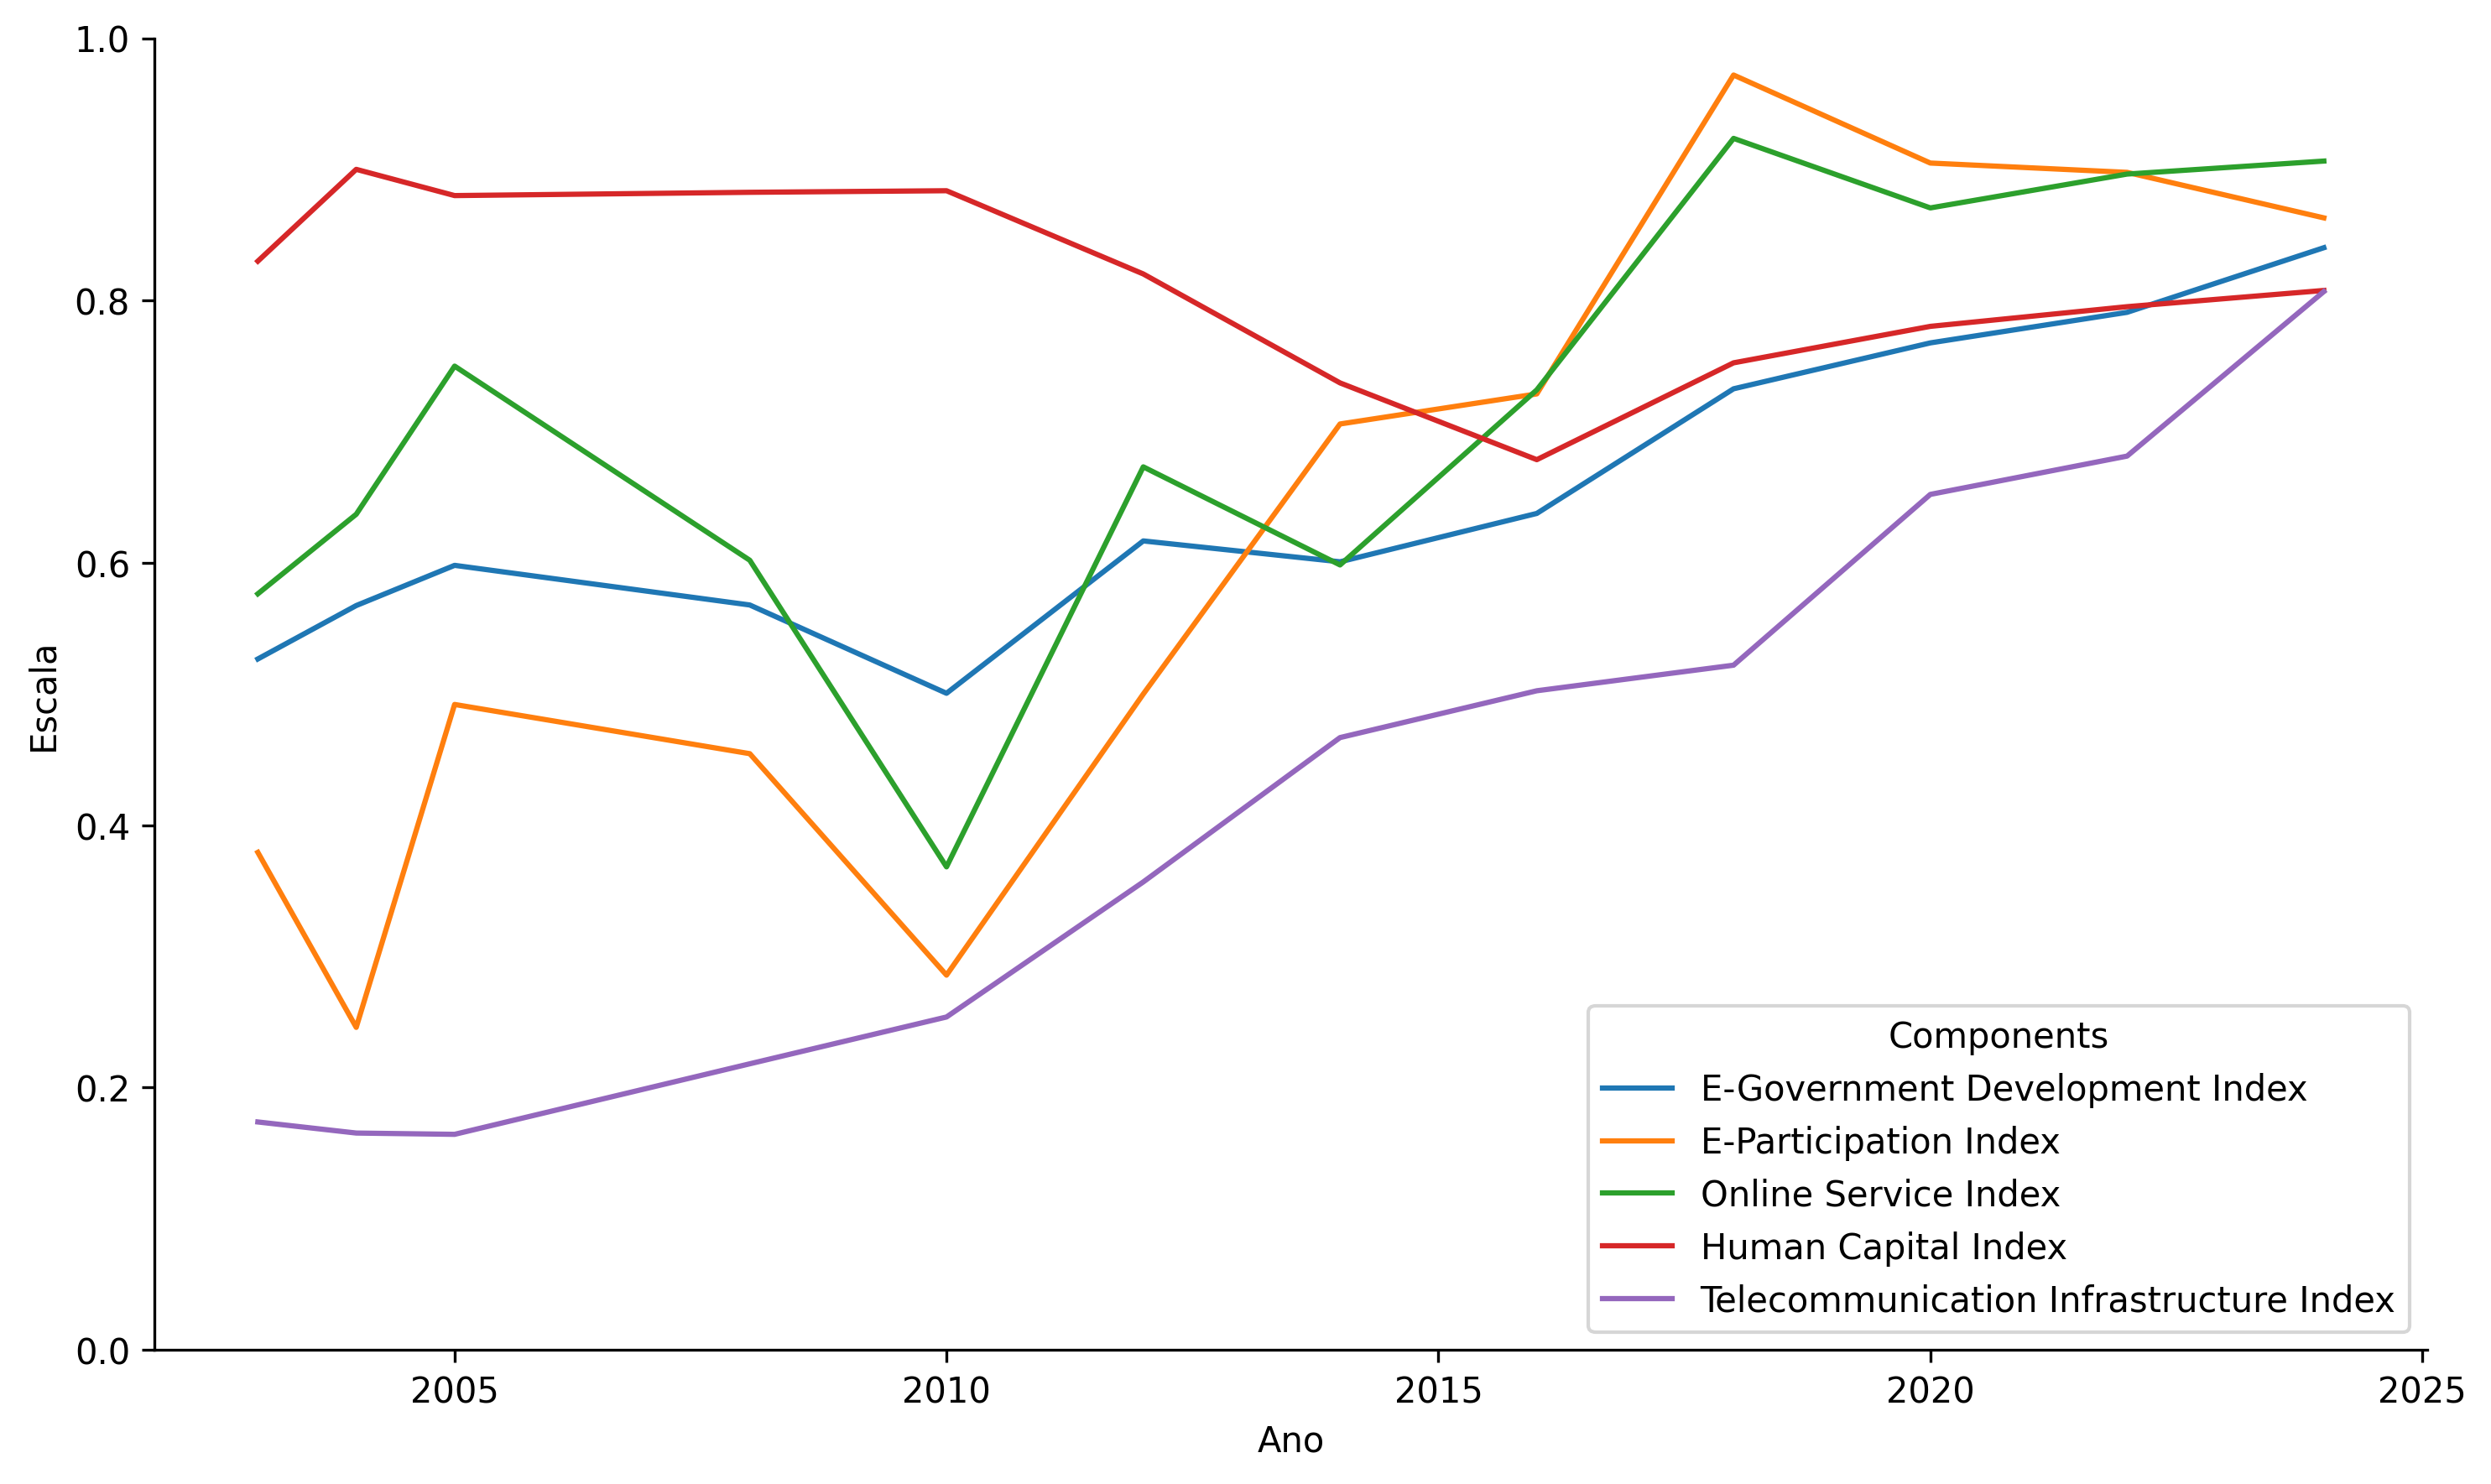
\includegraphics[width=1\linewidth]{figuras/egdi/lineplot_egdi_brasil.png}
	\label{fig:lineplot_egdi_brasil}
	\footnotesize{Fonte: baseado em \cite{ONU_EGDI_mapa}.}
\end{figure}

A maioria dos índices (\textbf{E-Government Development}, \textbf{Online Service},  \textbf{Human Capital} e, especialmente, o de  \textbf{Telecommunications Infrastructure}) apresenta uma tendência geral de crescimento ao longo do período, indicando uma melhoria na digitalização do governo e da sociedade brasileira.

Os  \textbf{E-Participation Index} e o \textbf{Online Service Index} mostram as maiores flutuações, com picos e quedas significativas em diferentes anos. Isso pode indicar variações nas políticas ou na implementação de serviços digitais e na participação cidadã.

\paragraph{E-Government Development Index} O índice principal mostra um crescimento constante, mas gradual, partindo de cerca de 0.5 em 2003 e atingindo mais de 0.8 em 2024. Sua trajetória reflete a média dos outros componentes, indicando uma evolução geral da capacidade do governo de fornecer serviços online.

\paragraph{E-Participation Index} Este índice é o mais volátil e o que apresenta o menor desempenho em grande parte do período. Ele tem um pico notável em 2005, seguido de uma queda e uma lenta recuperação. Isso sugere que a participação cidadã por meio de canais digitais é uma área que enfrenta desafios e flutuações, e seu desenvolvimento pode não ser tão linear quanto o de outros componentes.

\paragraph{Online Service Index} Após um pico inicial, este índice apresenta uma queda acentuada por volta de 2010, seguido de uma recuperação e um novo pico em 2018. Sua trajetória é irregular, o que pode refletir desafios na oferta de serviços públicos online. No entanto, ele termina o período em um nível alto, próximo do Human Capital Index.

\paragraph{Human Capital Index} Este índice mantém um nível consistentemente alto, geralmente entre 0.8 e 0.9, sendo o que mais se aproxima do valor máximo da escala. Apesar de algumas flutuações, ele demonstra que o Brasil possui um bom nível de capital humano para suportar o desenvolvimento do e-government, como educação e alfabetização digital.

\paragraph{Telecommunication Infrastructure Index} Este é o índice com o crescimento mais notável e constante. Ele parte de um patamar baixo (abaixo de 0.2 em 2003) e alcança o maior valor entre todos os índices no final do período (próximo de 0.8 em 2024). Isso sugere um avanço significativo na infraestrutura digital do país, como a expansão de banda larga e redes de telecomunicações.

\subsection{Comparando as métricas do Brasil com a média internacional de 2024}

